\pdfoutput=1
\documentclass[12pt]{report} 

\usepackage[
a4paper,
vmargin=2.5cm,
hmargin=3cm
]{geometry}


\renewcommand{\baselinestretch}{1.5}
\parskip=6pt

% DEFINICIÓN DE COLORES para portada y listados de código
\usepackage[table]{xcolor}
\definecolor{azulUC3M}{RGB}{0,0,102}
\definecolor{gray97}{gray}{.97}
\definecolor{gray75}{gray}{.75}
\definecolor{gray45}{gray}{.45}

% Soporte para GENERAR PDF/A --es importante de cara a su inclusión en e-Archivo porque es el formato óptimo de preservación y a la generación de metadatos, tal y como se describe en http://uc3m.libguides.com/ld.php?content_id=31389625. En la carpeta incluímos el archivo plantilla_tfg_2017.xmpdata en el que puedes incluir los metadatos que se incorporarán al archivo PDF cuando lo compiles. Ese archivo debe llamarse igual que tu archivo .tex. Puedes ver un ejemplo en esta misma carpeta.
\usepackage{amssymb}
\usepackage[a-1b]{pdfx}
\usepackage{hyperref}
% ENLACES

\hypersetup{colorlinks=true,
	linkcolor=black, % enlaces a partes del documento (p.e. índice) en color negro
	urlcolor=blue} % enlaces a recursos fuera del documento en azul

% EXPRESIONES MATEMATICAS
\usepackage{amsmath,amssymb,amsfonts,amsthm}

\usepackage{txfonts} 
\usepackage[T1]{fontenc}
\usepackage[utf8]{inputenc}

\usepackage[english]{babel} 
\usepackage[babel, english=american]{csquotes}
\AtBeginEnvironment{quote}{\small}

% Recipe for todos from http://tex.stackexchange.com/questions/9796/how-to-add-todo-notes
% \todo
\usepackage{xargs}                      % Use more than one optional parameter in a new commands
%\usepackage[pdftex,dvipsnames]{xcolor}  % Coloured text etc.
\usepackage[colorinlistoftodos,prependcaption,textsize=tiny]{todonotes}
\newcommandx{\unsure}[2][1=]{\todo[linecolor=red,backgroundcolor=red!25,bordercolor=red,#1]{#2}}
\newcommandx{\change}[2][1=]{\todo[linecolor=blue,backgroundcolor=blue!25,bordercolor=blue,#1]{#2}}
\newcommandx{\info}[2][1=]{\todo[linecolor=OliveGreen,backgroundcolor=OliveGreen!25,bordercolor=OliveGreen,#1]{#2}}
\newcommandx{\improvement}[2][1=]{\todo[linecolor=Plum,backgroundcolor=Plum!25,bordercolor=Plum,#1]{#2}}
\newcommandx{\thiswillnotshow}[2][1=]{\todo[disable,#1]{#2}}

% FVA: abbreviations 
\newcommand{\BT}{B.~Th.\xspace}


% diseño de PIE DE PÁGINA
\usepackage{fancyhdr}
\pagestyle{fancy}
\fancyhf{}
\renewcommand{\headrulewidth}{0pt}
\rfoot{\thepage}
\fancypagestyle{plain}{\pagestyle{fancy}}

\usepackage{titlesec}
\usepackage{titletoc}
\titleformat{\chapter}[block]
{\large\bfseries\filcenter}
{\thechapter.}
{5pt}
{\MakeUppercase}
{}
\titlespacing{\chapter}{0pt}{0pt}{*3}
\titlecontents{chapter}
[0pt]                                               
{}
{\contentsmargin{0pt}\thecontentslabel.\enspace\uppercase}
{\contentsmargin{0pt}\uppercase}                        
{\titlerule*[.7pc]{.}\contentspage}                 

\titleformat{\section}
{\bfseries}
{\thesection.}
{5pt}
{}
\titlecontents{section}
[5pt]                                               
{}
{\contentsmargin{0pt}\thecontentslabel.\enspace}
{\contentsmargin{0pt}}
{\titlerule*[.7pc]{.}\contentspage}

\titleformat{\subsection}
{\normalsize\bfseries}
{\thesubsection.}
{5pt}
{}
\titlecontents{subsection}
[10pt]                                               
{}
{\contentsmargin{0pt}                          
	\thecontentslabel.\enspace}
{\contentsmargin{0pt}}                        
{\titlerule*[.7pc]{.}\contentspage}  


% DISEÑO DE TABLAS. Puedes elegir entre el estilo para ingeniería o para ciencias sociales y humanidades. Por defecto, está activado el estilo de ingeniería. Si deseas utilizar el otro, comenta las líneas del diseño de ingeniería y descomenta las del diseño de ciencias sociales y humanidades
\usepackage{multirow} %permite combinar celdas 
\usepackage{caption} %para personalizar el título de tablas y figuras
\usepackage{floatrow} 
\usepackage{array} % con este paquete podemos definir en la siguiente línea un nuevo tipo de columna para tablas: ancho personalizado y contenido centrado
\newcolumntype{P}[1]{>{\centering\arraybackslash}p{#1}}
\DeclareCaptionFormat{upper}{#1#2\uppercase{#3}\par}

% Diseño de tabla para ingeniería
\captionsetup[table]{
	format=upper,
	justification=centering,
	labelsep=period,
	width=.75\linewidth,
	labelfont=small,
	font=small,
}

%Diseño de tabla para ciencias sociales y humanidades
%\captionsetup[table]{
%	justification=raggedright,
%	labelsep=period,
%	labelfont=small,
%	singlelinecheck=false,
%	font={small,bf}
%}


% DISEÑO DE FIGURAS. Puedes elegir entre el estilo para ingeniería o para ciencias sociales y humanidades. Por defecto, está activado el estilo de ingeniería. Si deseas utilizar el otro, comenta las líneas del diseño de ingeniería y descomenta las del diseño de ciencias sociales y humanidades
\usepackage{graphicx}
\usepackage{subcaption}
\graphicspath{{imagenes/}} %ruta a la carpeta de imágenes

% Diseño de figuras para ingeniería
\captionsetup[figure]{
	format=hang,
	name=Fig.,
	singlelinecheck=off,
	labelsep=period,
	labelfont=small,
	font=small		
}

% Diseño de figuras para ciencias sociales y humanidades
%\captionsetup[figure]{
%	format=hang,
%	name=Figure,
%	singlelinecheck=off,
%	labelsep=period,
%	labelfont=small,
%	font=small		
%}


% NOTAS A PIE DE PÁGINA
\usepackage{chngcntr} %para numeración contínua de las notas al pie
\counterwithout{footnote}{chapter}

% LISTADOS DE CÓDIGO
% soporte y estilo para listados de código. Más información en https://es.wikibooks.org/wiki/Manual_de_LaTeX/Listados_de_código/Listados_con_listings
\usepackage{listings}

% definimos un estilo de listings
\lstdefinestyle{estilo}{ frame=Ltb,
	framerule=0pt,
	aboveskip=0.5cm,
	framextopmargin=3pt,
	framexbottommargin=3pt,
	framexleftmargin=0.4cm,
	framesep=0pt,
	rulesep=.4pt,
	backgroundcolor=\color{gray97},
	rulesepcolor=\color{black},
	%
	basicstyle=\ttfamily\footnotesize,
	keywordstyle=\bfseries,
	stringstyle=\ttfamily,
	showstringspaces = false,
	commentstyle=\color{gray45},     
	%
	numbers=left,
	numbersep=15pt,
	numberstyle=\tiny,
	numberfirstline = false,
	breaklines=true,
	xleftmargin=\parindent
}

\captionsetup[lstlisting]{font=small, labelsep=period}
% fijamos el estilo a utilizar 
\lstset{style=estilo}
\renewcommand{\lstlistingname}{\uppercase{Código}}


%BIBLIOGRAFÍA - PUEDES ELEGIR ENTRE ESTILO IEEE O APA. POR DEFECTO ESTÁ CONFIGURADO IEEE. SI DESEAS USAR APA, COMENTA LAS LÍNEA DE IEEE Y DESCOMENTA LAS DE APA. Si haces cambios en la configuración de la bibliografía y no obtienes los resultados esperados, es recomendable limpiar los archivos auxiliares y volver a compilar en este orden: COMPILAR-BIBLIOGRAFIA-COMPILAR
% Tienes más información sobre cómo generar bibliografía en http://tex.stackexchange.com/questions/154751/biblatex-with-biber-configuring-my-editor-to-avoid-undefined-citations , https://es.sharelatex.com/learn/Bibliography_management_in_LaTeX y en http://www.ctan.org/tex-archive/macros/latex/exptl/biblatex-contrib
% También te recomendamos consultar la guía temática de la Biblioteca sobre citas bibliográficas: http://uc3m.libguides.com/guias_tematicas/citas_bibliograficas/inicio

% CONFIGURACIÓN PARA LA BIBLIOGRAFÍA IEEE
\usepackage[backend=biber, style=ieee, isbn=false,sortcites, maxbibnames=5, minbibnames=1]{biblatex} % Configuración para el estilo de citas de IEEE, recomendado para el área de ingeniería. "maxbibnames" indica que a partir de 5 autores trunque la lista el primero (minbibnames) y añada "et al." tal y como se utiliza en el estilo IEEE.

%CONFIGURACIÓN PARA LA BIBLIOGRAFÍA APA
%\usepackage[style=apa, backend=biber, natbib=true, hyperref=true, uniquelist=false, sortcites]{biblatex}
%\DeclareLanguageMapping{spanish}{spanish-apa}

\addbibresource{bibliografia/bibliografia.bib} % llama al archivo bibliografia.bib que utilizamos de ejemplo


%-------------
%	DOCUMENTO
%-------------
\graphicspath {{Figuras_tfg/}}

\begin{document}
\pagenumbering{roman} % Se utilizan cifras romanas en la numeración de las páginas previas al cuerpo del trabajo
	
%----------
%	PORTADA
%----------	
\begin{titlepage}
	\begin{sffamily}
	\color{azulUC3M}
	\begin{center}
		\begin{figure}[H] %incluimos el logotipo de la Universidad
			\makebox[\textwidth][c]{
\includegraphics[width=16cm]{Figuras_tfg/Portada_Logo.png}}
		\end{figure}
		\vspace{2.5cm}
		\begin{Large}
			Bachelor's Degree in Telecommunication Engineering\\			
			Academic Year 2018-2019\\
			\vspace{2cm}		
			\textsl{Bachelor Thesis}
			\bigskip
			
		\end{Large}
		 	{\Huge ``Triangulos Entropicos''}\\
		 	\vspace*{0.5cm}
	 		\rule{10.5cm}{0.1mm}\\
			\vspace*{0.9cm}
			{\LARGE Adrian Manuel de Luis García}\\ 
			\vspace*{1cm}
		\begin{Large}
			1st Tutor complete name\\
			2nd Tutor complete name\\
			Place and date\\
		\end{Large}
	\end{center}
	\vfill
	\color{black}
	% si nuestro trabajo se va a publicar con una licencia Creative Commons, incluir estas líneas. Es la opción recomendada.
	
\includegraphics[width=4.2cm]{imagenes/creativecommons.png}\\  %incluimos el logotipo de creativecommons
	\emph{[Include this code in case you want your Bachelor Thesis published in Open Access University Repository]}\\ % BORRAR ESTA LÍNEA
	This work is licensed under Creative Commons \textbf{Attribution – Non Commercial – Non Derivatives}
	\end{sffamily}
\end{titlepage}

\newpage %página en blanco o de cortesía
\thispagestyle{empty}
\mbox{}

%----------
%	RESUMEN Y PALABRAS CLAVE
%----------	
\renewcommand\abstractname{\large\uppercase{Summary}}
\begin{abstract}
\thispagestyle{plain}
\setcounter{page}{3}
	
The aim of this report is to analyse the performance of Entropy Triangles when applied to typical Deep Neural Datasets.
	
	\textbf{Keywords:}
	% Escribir las palabras clave aquí
	
	\vfill
\end{abstract}
	\newpage % página en blanco o de cortesía
	\thispagestyle{empty}
	\mbox{}


%----------
%	DEDICATORIA
%----------	
\chapter*{Dedication}

\setcounter{page}{5}
	
	% ESCRIBIR LA DEDICATORIA AQUÍ	
		
	\vfill
	
	\newpage % página en blanco o de cortesía
	\thispagestyle{empty}
	\mbox{}
	

%----------
%	ÍNDICES
%----------	

%--
%Índice general
%-
\tableofcontents
\thispagestyle{fancy}

\newpage % página en blanco o de cortesía
\thispagestyle{empty}
\mbox{}

%--
% Índice de figuras. Si no se incluyen, comenta las líneas siguientes
%-
\listoffigures
\thispagestyle{fancy}

\newpage % página en blanco o de cortesía
\thispagestyle{empty}
\mbox{}

%--
% Índice de tablas. Si no se incluyen, comenta las líneas siguientes
%-
\listoftables
\thispagestyle{fancy}

\newpage % página en blanco o de cortesía
\thispagestyle{empty}
\mbox{}


%----------
%	TRABAJO
%----------	
\clearpage
\pagenumbering{arabic} % numeración con múmeros arábigos para el resto de la publicación	

\chapter{Introduction}

Information has usually been referred as one of the key aspects that all learning system need in order to increase its capabilities and improve its performance. This is specially relevant for the data analytics field and the process of designing machine learning applications, where many experts usually refer to information as a powerful metric to indicate the success of their architecture at solving a particular problem. Due to the plethora of works already available online to master and use different techniques, the goal of this work is to asses the capabilities of these techniques and discuss its informational properties. \par
\setlength{\parindent}{10ex}
During the last few years, the topic of Big Data has become increasingly more important in our society. It is currently being used or developed in almost every industry in the world[1](Quote article to reinforce my position on this matter?) and it is growing faster every day. While methods like Deep Neural Networks are beginning to be widespread available,  researchers tend to use the same approaches and steps to get their results. Rather than trying new methods, it is an industry standard to use a certain set of techniques when presented with a type of problem and then to try to optimise it. It is just assumed that these methods are powerful enough to find a suitable answer.  \par
An instance of this model can be found on [2], where each block represents a different function inside an end-to-end informational model. We can only take measures outside each of the blocks and the contents or the methods being used inside are outside of the scope of the task. By not being able to access each one of the blocks to evaluate the processes happening inside of them, we are only fixing or changing values outside of them to try to improve our reuslts. \par

\begin{figure}[h]
\begin{subfigure}{1\textwidth}  
 \centering
  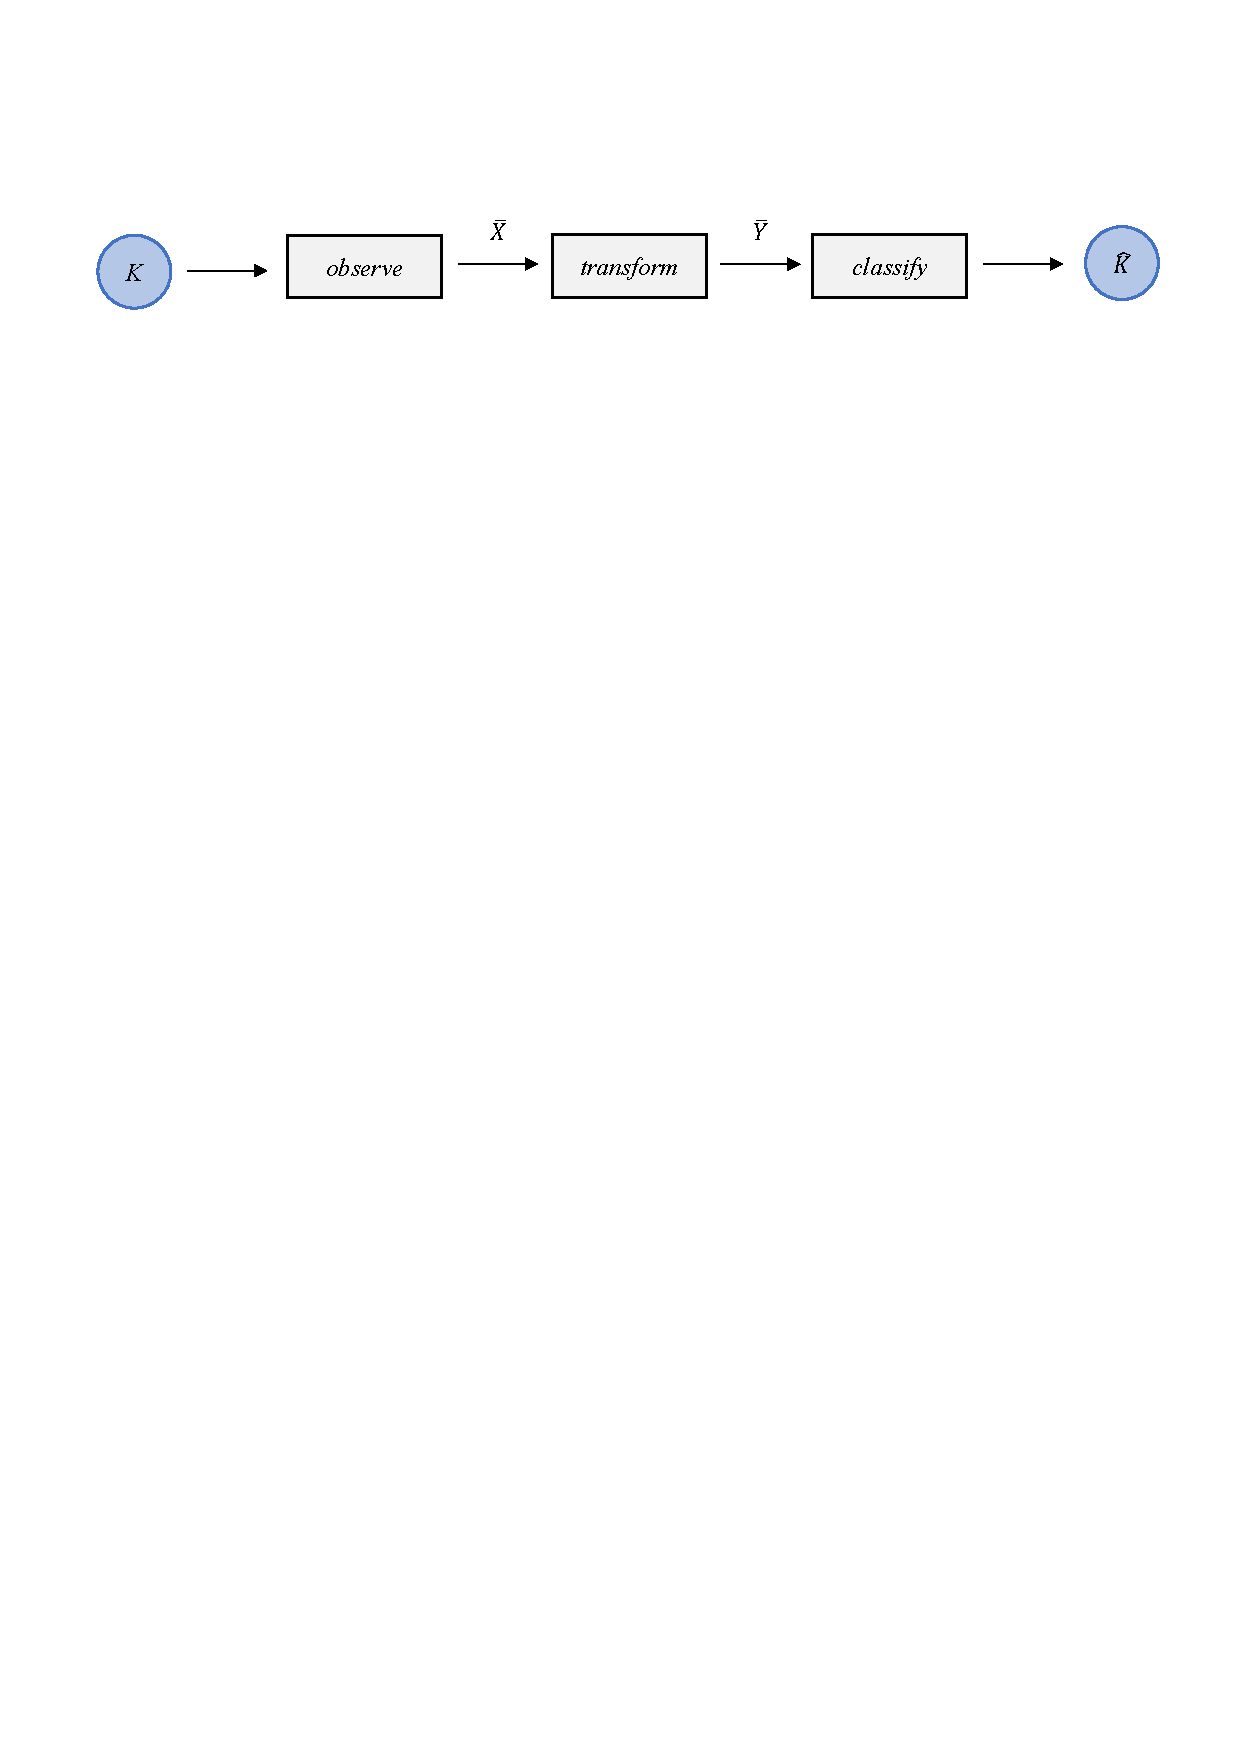
\includegraphics[width=16cm]{Figuras_tfg/Figura1_tfg}
  \caption{Conceptual representation of a classification process mimicking a communication scheme of boxes.}
 \label{fig:fig1a} 
\end{subfigure}%  

\begin{subfigure}{1\textwidth} 
  \centering
  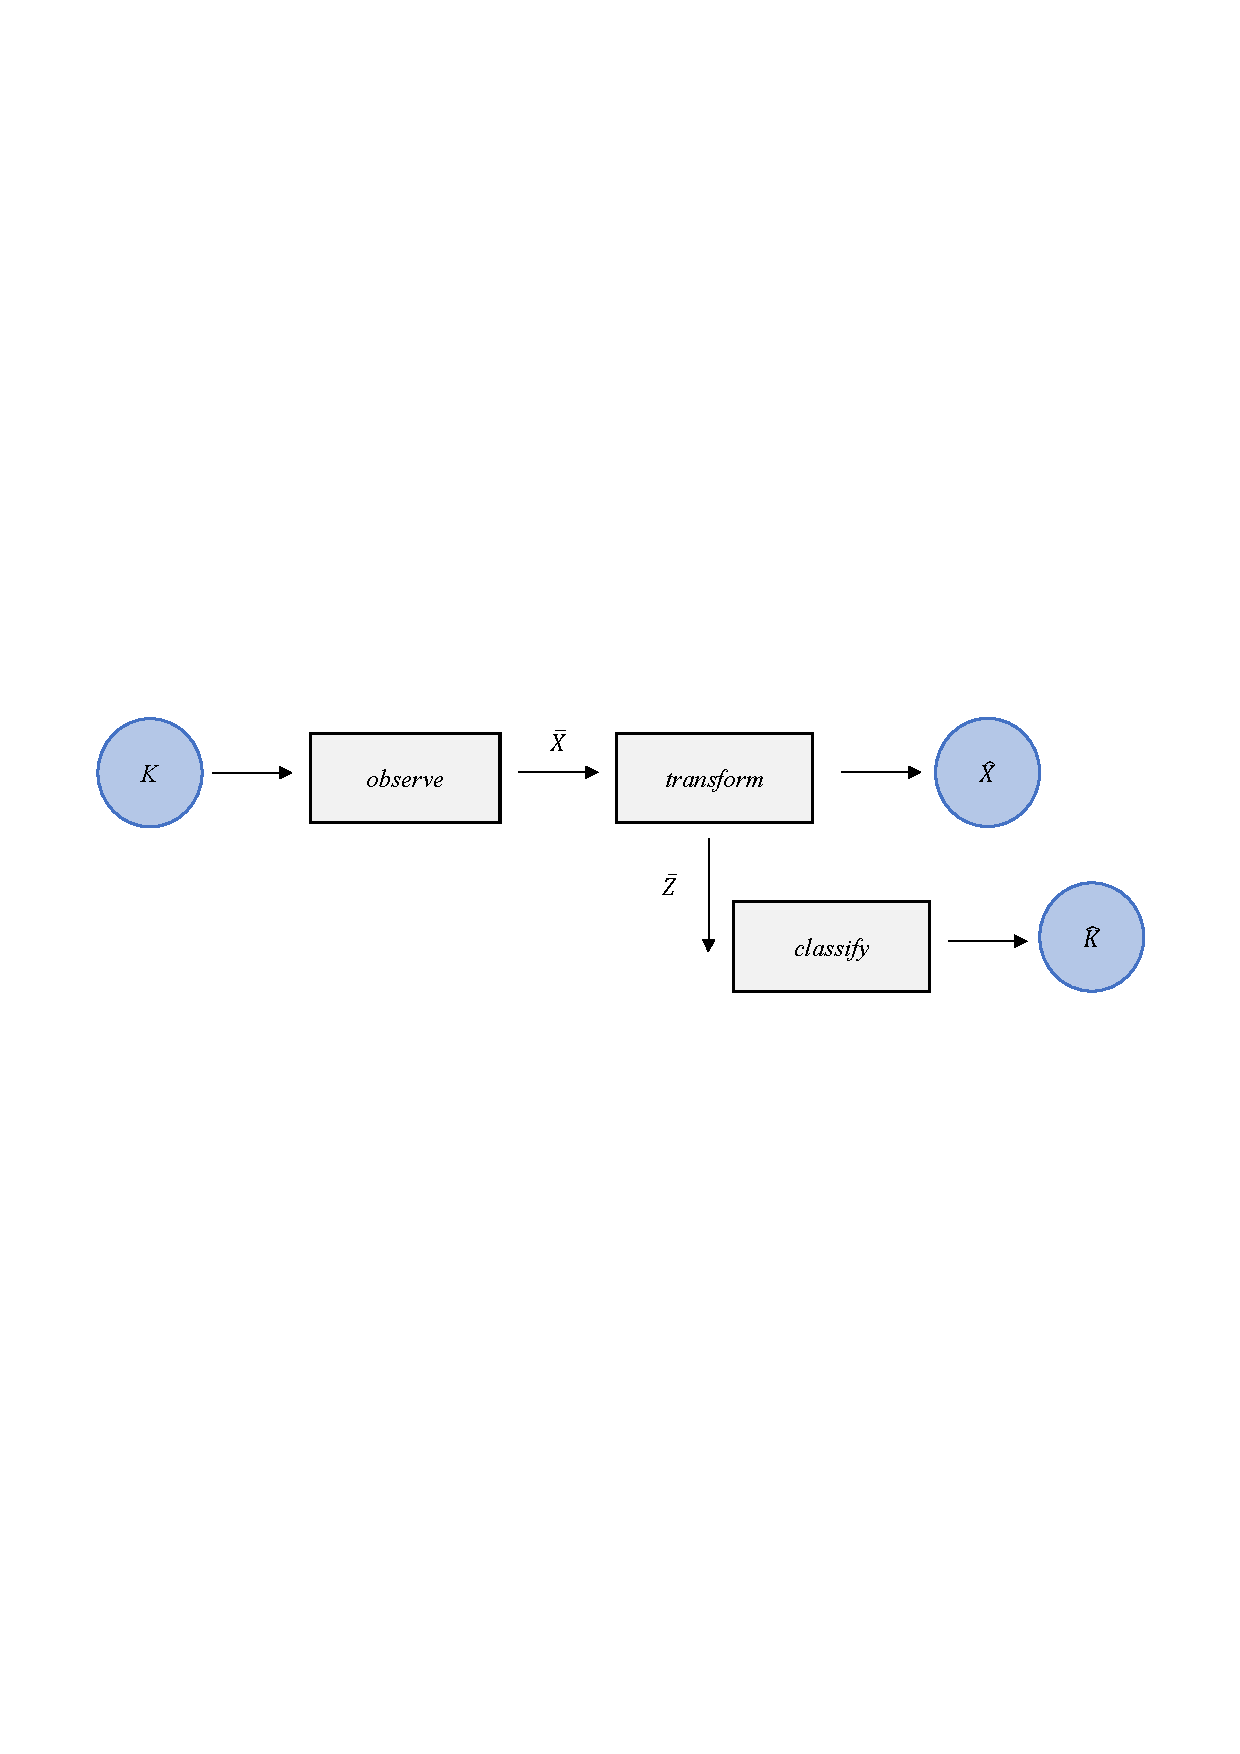
\includegraphics[width=16.5cm]{Figuras_tfg/Figura1_1_tfg}
  \caption{Our end-to-end scheme uses the information regarded from inside the transformation block and we then produce two outputs. First, the predicted (X) which we can use to measure our transformation accuracy. Secondly, the (Z), which contains compressed information about (X)}
  \label{fig:fig1a} 
\end{subfigure}%  
\caption{Comparison between the classical view of a supervised classification in (a) versus the the model implemented for the purpose of this work in (b).}
\label{fig:fig1}
\end{figure}


The model that I will be implementing will be an adaptation of the scheme on Figure \ref{fig:fig1a}. To further investigate on the boundaries of Information transmission , I will be using an (en negrita) Autoencoder to test the Information Bottleneck Principle. \par

In this report, I designed the following model which provides reliable information about the process of data compression and the limits of quantifiable information: \par

- We have a random source $K$ generating random observations. Through a process of measurements, our system then will be provided with other random observations $\hat{X}$. \\
-The observations outputted are then fed to the Autoencoder, which will then reduce the (X con gorro) into another vector $Z$with a different length but retaining the information from the input vector in a compressed from. \\
-The Autoencoder also provides with an output, which should be a reconstruction of the observations used to feed the Deep Learning structure. \\
-The $Z$ is then used for the classifying task of choice to output the predicted labels. \par

Note that Figure \ref{ifg:fig1a} follows a similar model than Figure \ref{ifg:fig1}, but its transformation block is used to access the inside content of it rather than to provide a typical representation of an end-to-end transformation scheme. Although both of them typify a MIMO (Multiple Input Multiple Output) block, the Autoencoder is essentially an unsupervised transformation method, while the transformation block can be either composed by supervised or unsupervised task. The inner workings and different features of the Autoencoder will be explained on Section 2.1. \par

Here is where I explain further the concepts to be used on this Final Degree Project and the rest of methods to use on it \par

\chapter{Methods}
\section{The Autoencoder}
\subsection{Deep Neural Networks}

To clearly explain what an Autoencoder is, we must first lay the foundations of one of its core concepts: Deep Neural Networks. DNN constitute the basis of Deep Learning and they have proven themselves to be complex enough to tackle many of the data challenges of today. \par

\begin{figure}[H]
\begin{subfigure}{0.65\linewidth}  
 \centering
  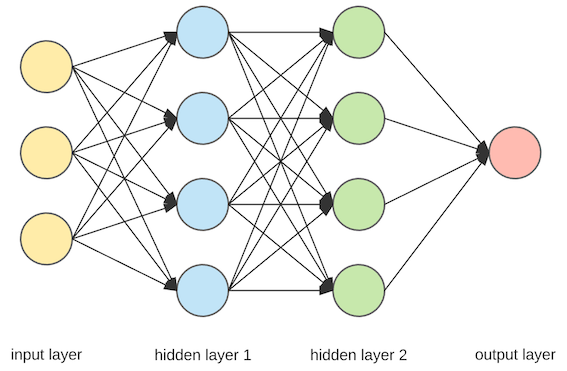
\includegraphics[width=\linewidth]{Figuras_tfg/Figure2_tfg}
  \caption{Basic depiction of a simple DNN composed by two hidden layers and a single 2-input/1-output system.}
  \label{fig:fig2a} 
\end{subfigure}

\begin{subfigure}{0.65\linewidth} 
  \centering
  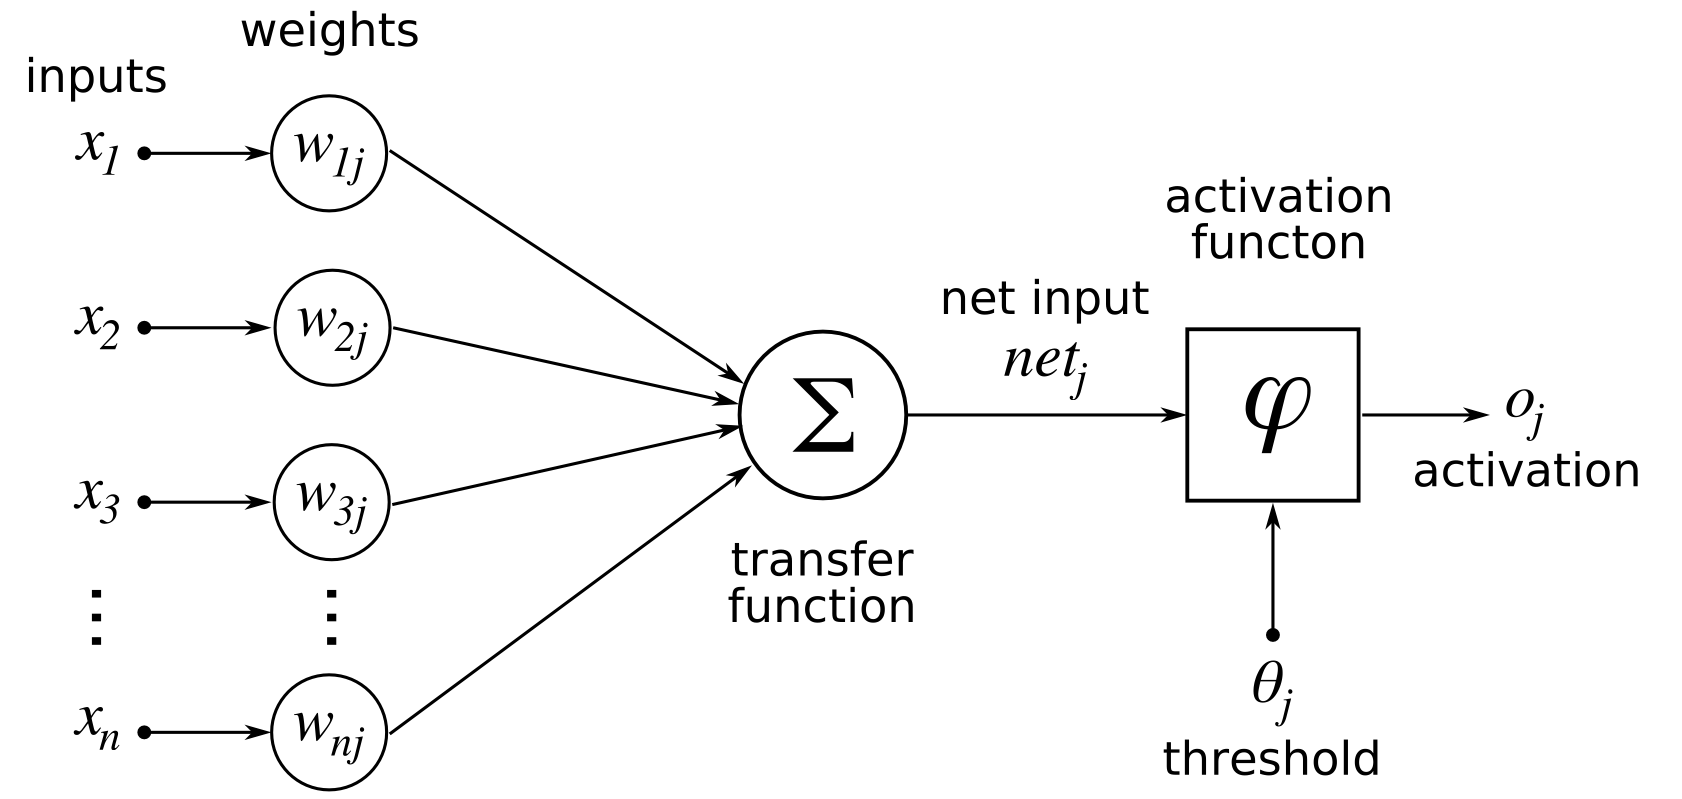
\includegraphics[width=\linewidth]{Figuras_tfg/ArtificialNeuronModel_english.png}
  \caption{Normal architecture of an artificial neuron.}
  \label{fig:fig2b} 
\end{subfigure}
  \caption{Basic depiction of a simple DNN composed by two hidden layers and a single 2-input/1-output system.}
 \label{fig:fig2}
\end{figure}

By analysing Figure2a, it can be noted that DNNs are comprised of multiple layers of units (or neurons) with a relatively small computing power which is calculated using the weights from previous layers combined with an activation function as seen on and \ref{fig:fig2}. It also has an input (usually denoted as X) which is feed-forwarded to the hidden layers in the network and subsequently transformed into an output (commonly denoted as Y). 

\begin{equation}\label{eq:artificial neuron}
Output = f( bias_j + \sum_{i = 0}^{n} w_{i}*x_i ) 
\end{equation}


Neurons inside of the network can be modelled according to different types, although in this report we will be only taking into account two of them: the sigmoid $f(x) = \frac{1}{1 - e{-x}}$ (Figure a) and the relu $f(x) = max(0,x)$(Figure b) neurons. I chose to use this type of neurons because their activation functions are excellent for minimizing the reconstruction loss inside of the autoencoder. \newline

\begin{figure}[H]
 \begin{minipage}{.5\textwidth}
        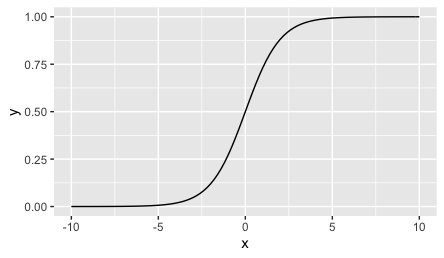
\includegraphics[scale=.5]{Sigmoid_function}
 \end{minipage}%
 \begin{minipage}{.5\textwidth}
        \begin{flushright}
               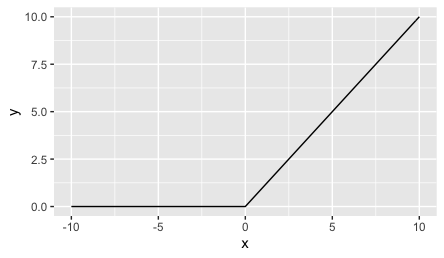
\includegraphics[scale=.5]{Relu_function}  
        \end{flushright} 
    \end{minipage}  
    \caption{The left graph represents a Sigmoid function, while on the right there is a Relu function}
 \label{fig:fig3}
\end{figure}

As it can be seen on Figure\ref{fig:fig3} , the Relu function has a relatively simple representation, which makes it less computationally expensive when compared with the Sigmoid. The Sigmoid function is also very useful since it takes values between 0 and 1, which makes it specially useful when we want to place a classifier as the next task after the transformation.\par 

Once a certain DNN structure has been activated, the neurones inside of the network will start to propagate the information through it in a non-linear manner in order to try to achieve a given stablished task, which in our particular case consists in transforming the representation of our input into a smaller but informationally more compressed form. Other experts can use the same principles to achieve other goals including decision-making, visualisation,....etc.\par

\subsection{Information Bottleneck Principle}

The architecture of the Autoencoder is based upon the IB, a method proposed in [paper which mentions it] whose principle relies on extracting the relevant information that an input random variable X contains about another output random variable Y. If we assume that there is some type of statistical dependency between X and Y, the relevant information can be defined as I(X;Y).\par

If we want to obtain the optimal representation of X we would want to capture the relevant information of X that contributes to an accurate prediction of Y. This term is known as the (minimal sufficient statistics), or simply just the mapping of X that retains I(X;Y).\par

During the learning process, and as depicted in figure (DNN self-explanatory figure), DNN only have access to the information that has been transferred to them via the previous layers of the system. This has a big effect on out network: the information not processed on the last immediate layer is essentially lost. This is the main reason why every layer should attempt to maximise I(Y;hi) while trying to minimise the I (hi-1;hi). Here, it is important to consider then that we want to reduce the length of the layer to the minimum possible without affecting the the predictive features of our model.

Each layer of our model should require shorter descriptions than the previous ones, being the first one with the longest description and the least compression. It must also be noted that every model will require a different set of layers an architecture to fit its computational needs to the optimal level.

\subsection{The Autoencoder Architecture}

Applying the concepts introduced on both previous sections (the two sections appearing before this one, when  i figure the final numbers ), the autoencoder comes as a mixture of them. Figure [] below presents it as a three part structure: A encoder, the middle layer and finally the decoder. \par

\begin{figure}[H]
 \centering
  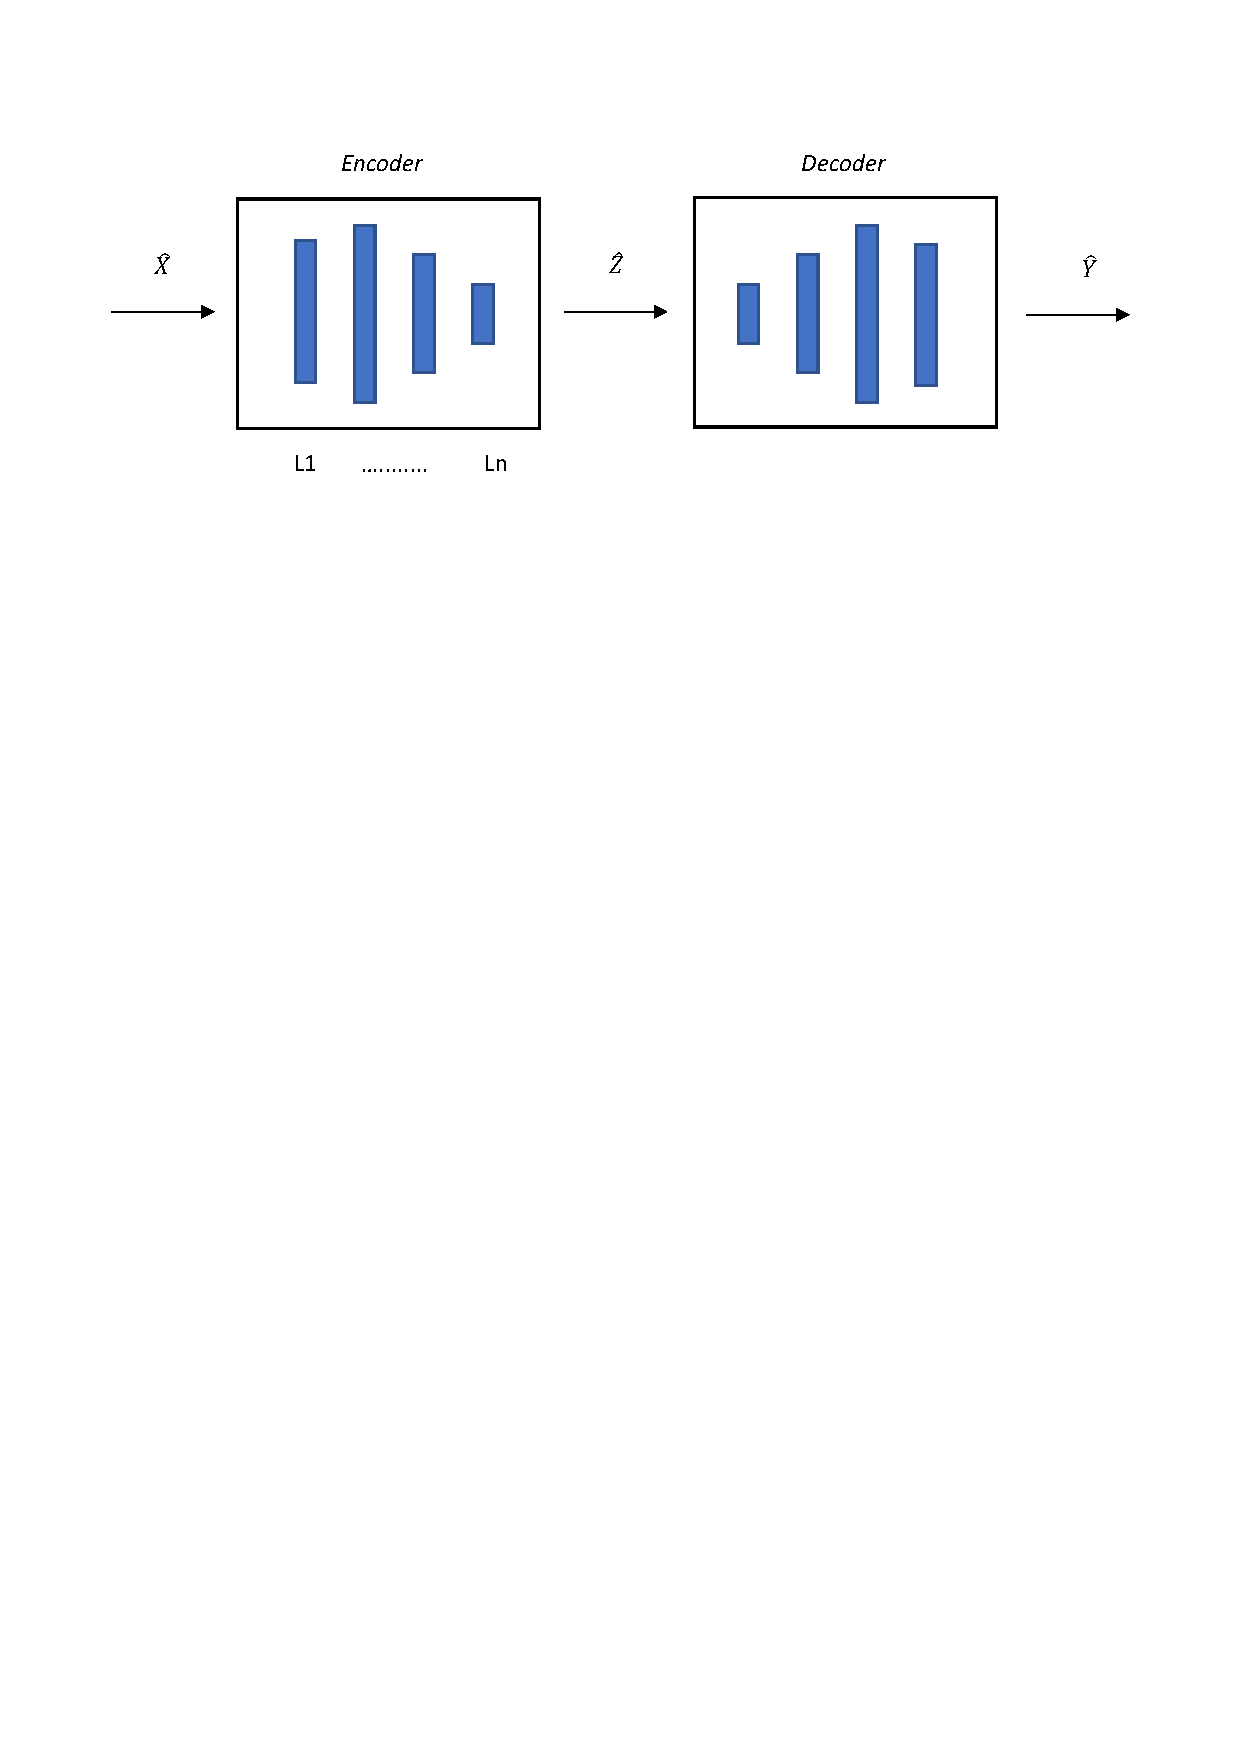
\includegraphics[width=16cm]{Figuras_tfg/Figura_autoencoder}
  \caption{Taking into account the Figure \ref{fig:fig1a}, this diagram depicts the inside of the transformation box. Both the Encoder and the Decoder have symmetric shapes, as well as an expansion layer (the second one in the encoder, the previous one in the decoder) whose goal is to separate the qualities of our data as sort of a preparation for the compression.}
 \label{fig:figure_autoencoder}
\end{figure} 

The theory of the autoencoder has been around since the 1980s (put as a reference the article where it is first presented). As seen in Figure[], the autoencoder's goal is not only to copy the input data and then transmit it through the network, but to retain the most important features of the data fed to it and to try to optimise the process of learning them. For the purpose of my research, I will only be considering the back-propagated autoencoders, although it must be noted that other variances of them exist, such as the recirculated autoencoders. \par

In our case, we will be also using an undercomplete autoencoder. Most of the types an autoencoder is employed, it is usually more interesting to focus on its data compression capabilities rather than trying to copy the input onto the output. That is why we want to force the autoencoder to provide us with a smaller dimension on the input data X in the output on the encoder, which for the purpose of this report we will denominate as Z. The learning process, as described in (paper where i got the equation from) tries to minimise the given equation: \par

\begin{equation}\label{eq:artificial neuron}
L(x,g(f(x)))
\end{equation}
The L function is a loss function, which penalises $g(f(x))$ for being dissimilar from $x$.

One thing to take into account when designing an autoencoder is that giving too much capacity to its layers can be counterproductive to the learning task. This means that when given too much capacity to work with they will tend to learn to avoid extracting information and rather to just copy the information, which is an undesirable outcome. On the other hand, trying to set an encoder to code the input signal into a single dimension could result in the loss of valuable information. Even with a very powerful decoder a very optimised autoencoder will struggle to perform this task, specially when introducing very big sets data as the input. \par

Taking into account this description, the general rule to design it is just by using trial and error. As we will see on Section3, where I will be discussing the implementation of the autoencoder, you can try different setups to reach the optimum middle layer size which accomplishes that there is no trade-off between augmenting its size and keeping its actual capabilities. The Tensorflow python tool provides us with the accuracy and loss variables that the autoencoder is generating on each training epoch to check if your architecture is fulfilling your requirements. For the purpose of this report, we will not only taking into account those parameters, but we will also be using a tool to ensure that it transfering the higher quantity of information possible: The entropy triangle.

\subsection{The Entropy Triangle}
\subsubsection{Introduction}

In the previous section I have talked about how accuracy can be used to asses the validity of our model. In reality, the accuracy value can be somewhat misleading depending of the task that we are implementing it to check if we are carrying out our data analysis correctly. This statement is specially true when talking about Classification.\par

The usage of data classification has greatly improved in the past years. Nowadays, there are multiple papers discussing how it can be used in a wide range of topics, from the medical field to the face recognition task. That is why it is specially important to correctly address the scope of your task and how accurately does your model predict in your pre-defined scenarios.\par

\begin{figure}[H]
 \centering
  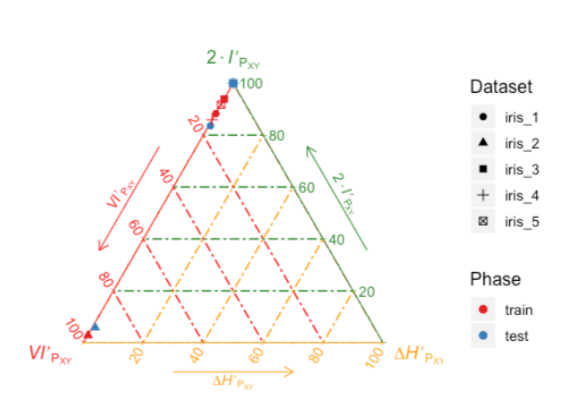
\includegraphics[width=15cm]{Figuras_tfg/Example_ET}
  \caption{Example of use of a typical Entropy Triangle. In this case, a Knn classification method is being tested in the triangle.}
 \label{fig:figure_example_et}
\end{figure} 

The real question comes when you have your results and you try to wrap your mind around them. In [paper donde se discute ese tema] a very important reality is shown: the accuracy performance criterion is a very intuitive but ineffective tool. Another highly important concept is introduced here: the accuracy paradox.\par  

The accuracy paradox shows some of the defects that classifiers have been presenting for a long time now . For example, in some cases predictive classifiers which have given a lower accuracy power have also proven to display a higher predictive accuracy that other with a higher accuracy. The reason being most of the times is that we have trained our classifier with a single class that contains the majority of the data. In those cases, our classifier will just assign all of the input values to belong to the majority class since that is where the greater probability lies upon. This one is a very easily identifiable case of an imbalanced training data set. Moreover, since most of the times our data is gathered in controlled conditions, we risk the problem of this issue showing up more than we would wish to.\par

Once it is realised that the methods previously employed can lead to disingenuous results, a new realisation arrises: there is a need for a better measure of the classifier. As seen in  [], the Entropy Triangle and its features show some numeric example that fit the requirements and scope of our task, so I will be using it. Bur firstly, I will explain the basics of its functionalities.\par

\subsubsection{Architecture}

The Entropy Triangle was introduced in ... as a way of solving the problems introduced in the previous section. We consider the transmission of information through a channel as two random variables, named X for the input and Y for the output. Note that on Figure\ref{fig:fig1} we used a different naming standard, K and $\hat{K}$,but the new reference names are now implemented for the sake of easier computations. In Figure we can see a classical information-diagram ... which simply show the entropy relationship between X and Y or $P_xy$. From that Figure we can also asses some equations from it:\par

The Mutual Information, which quantifies the stochastic force between $P_X$ and $P_Y$ appears twice in the diagram both as:
\begin{equation}\label{eq:mutual_information_1}
MI_{P_{XY}} = H_{P_X * P_Y} - H_{P_{XY}}
\end{equation}
and,
\begin{equation}\label{eq:mutual_information_2}
MI_{P_{XY}} = H_{P_X} - H_{P_{X|Y}}
\end{equation}

The Virtual Information or variation of information are embodied by the sum of the two red areas and represents the residual entropy, which is not used in the binding of the variables:

\begin{equation}\label{eq:virtual_information}
VI_{P_{XY}} = H_{P_{Y|X}} + H_{P_{X|Y}}
\end{equation}

And both equations mentioned before together with $\Delta H_{P_{X} * P_{Y}}$, which represents the divergence between the joint distribution where $P_X$ and $P_Y$ are independent and the uniform distributions with the same cardinality of events as the previously mentioned $P_X$ and $P_Y$, form:

\begin{equation}\label{eq:uniform_entropy_x_y}
H_{U_{X} * U_{Y}} = \Delta H_{P_{X} * P_{Y}} + 2 * MI_{P_{XY}} + VI_{P_{XY}}
\end{equation}

In which case $H_{U_{X} * U_{Y}}$ is the outer rectangle with both the uniform distributions of the input and the output.

Once we have obtained equation\ref{eq:uniform_entropy_x_y} we will normalise it using the  $H_{U_{X} * U_{Y}}$ and thus forcing the variables involved in our calculations to be bounded by 0 and 1, as it can be seen on:

\begin{equation}\label{eq:normalised_uniformed}
1 = \Delta'H_{P_{X} * P_{Y}} + 2 * MI'_{P_{XY}} + VI'_{P_{XY}} 
\end{equation}
Which also will wield the following equation:
\begin{equation}\label{eq:complex_space_equation}
0 \leq \Delta'H_{P_{X} * P_{Y}}, MI'_{P_{XY}}, VI'_{P_{XY}}  \leq 1
\end{equation}
\newline
\begin{figure}[H]
 \centering
  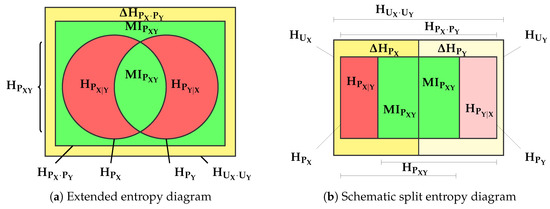
\includegraphics[width=14cm]{Figuras_tfg/ET_Diagram}
  \caption{Diagram representing an ET applied to a bivariate distribution.}
 \label{fig:figure_diagram_et}
\end{figure} 


By applying both equations \ref{eq:normalised_uniformed} and \ref{eq:complex_space_equation} we will get a point in the normalised space  $\Delta'H_{P_{X} * P_{Y}} x 2*MI'_{P_{XY}} x VI'_{P_{XY}}$. Each $P_{XY}$ can be characterised as $F(P_{XY}) = [\Delta'H_{P_{X} * P_{Y}},2*MI'_{P_{XY}},VI'_{P_{XY}}] $. The resulting diagram will be an equilateral triangle, where the coordinates are $F(P_{XY})$ and every bivariate distribution is shown as a point in the diagram. Every zone of the triangle has certain characteristics related to it. \par

We can also divide equation \ref{eq:uniform_entropy_x_y} to obtain new representations of the split balance equations with respect to $X$ and $Y$,

\begin{equation}\label{eq:entropy_x_balance}
H_{U_{X}} = \Delta H_{P_{X}} + MI_{P_{XY}} + H_{P_{X|Y}}  -> 1 = \Delta H'_{P_{X}} + MI'_{P_{XY}} + H'_{P_{X|Y}}
\end{equation}
and,
\begin{equation}\label{eq:entropy_y_balance}
H_{U_{Y}} = \Delta H_{P_{Y}} + MI_{P_{XY}} + H_{P_{Y|X}}  -> 1 = \Delta H'_{P_{Y}} + MI'_{P_{XY}} + H'_{P_{Y|X}}
\end{equation}

Both equations are normalised by using both $H_{U_{X}}$ and $H_{U_{Y}}$ respectibly. Now, we have new representations for $X$ and $Y$ in the 2-simplex triangle created before. The representation seems to split in two and have $F(P_X) = [\Delta'H_{P_{X}},MI'_{P_{XY}},H'_{P_{X|Y}}] $ and $F(P_Y) = [\Delta'H_{P_{Y}},MI'_{P_{XY}},H'_{P_{Y|X}}]$ coordinates.\newline

\begin{figure}[H]
 \centering
  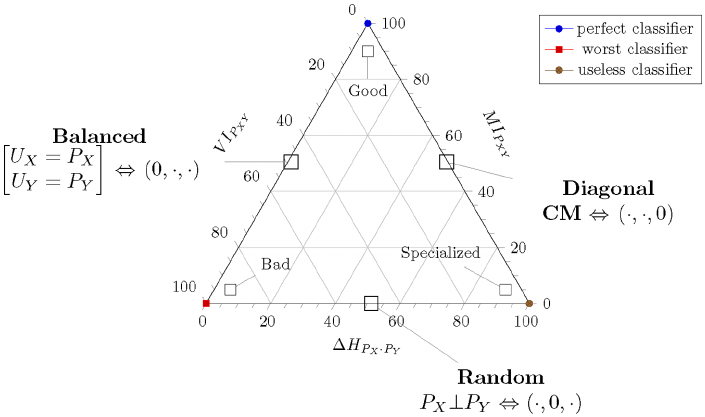
\includegraphics[width=15cm]{Figuras_tfg/ET_Labelled.png}
  \caption{Schematic of an Entropy Triangle. The labels are placed close to the side of the triangle that is related to the feature mentioned in it.}
 \label{fig:figure_labelled_et}
\end{figure} 

Most of the equations included here can be found in [] which discusses most of the points mentioned here along with some examples of use and much more information on the tool and different implications of its use. \par

The triangle itself works as a great tool to characterise the performance of your model. The position of the coordinates assesses the quality of your classifier. It can be appreciated from Figure \ref{fig:figure_labelled_et} that classifiers which are at the apex or close to it obtain the highest accuracy possible on balanced datasets and transmit a lot of mutual information, which makes them the best classifiers possible. On the other hand, when the coordinates of the classifier are very close to the left apex, we will be working with balanced data but the classifier will be doing a very bad work with it, we are dealing with the worst classifier. Finally, those who are located at the right apex or close to it represent the accuracy paradox mentioned before, which a highly specialised classifier which tries to work with very unbalanced data.\par

One example of use of the Entropy Triangle which appears on Section3 together with the results of the experiments would be to use the true labels $K$ and the predicted labels $\hat{K}$ to generate a confusion matrix. Information to be fed the ET can then be calculated with it and thus provide the diagram with enough materials to be created. The tool can then be used for exploratory analysis and help provide visual data to assess the feasibility of the task and its effectiveness.\par

\section{Principal Component Analysis}
\subsection{Description}
The Principal Component Analysis in a statistical procedure based on orthogonal transformations to convert observations of possibly uncorrelated variables into sets of linearly uncorrelated variables called (principal components). The transformation is performed in such a way that the first component has the largest possible variance, with each succeeding component having the highest variance taking into account that it has to be orthogonal to the preceding components. We will finally end up with a set of of vector which are uncorrelated. Due to the nature of the transformation, PCA can be affected by any type of scaling of the original dataset. \par

PCA is used in the data analysis field for exploratory data analysis or to make predictive models. It can be used to visualise the genetic distance between populations of data. Results from the PCA are usually discussed taking into account their components. Other characteristics include:

\begin{description}
	
\item[$\bullet$] PCA is a simple eigenvector-based multivariate analysis. This is specially important to our task since this operation can help us discern the real structure of the data. It can also reduce the dimensionality of the data to view its most informative components and features.

\item[$\bullet$] It resembles factor analysis. Both of them are used to describe the variability of the data and reduce the dimensionality of the data, but aim to use different techniques to reach that goal.

\item[$\bullet$] It also resembles canonical correlation analysis. While CCA tries to describe the cross-variance between two datasets, PCA defines the variance of a single dataset by using an orthogonal coordinate system.

\end{description}

\subsection{PCA and Information Theory}

Our goal when using PCA in this project is to try to give other examples of data transformation to compare the results of the Autoencoder with another widely used tool in the data science field. At the same time, we want the Information theory to be implicit on both methods used so that the outcome can be correctly compared when using the Entropy Triangle.\par

PCA fullfils our requirements by trying to minimise the informational losses. If we assume our model vectors to be defined by the  following equation :

\begin{equation}\label{eq:pca_equation}
x = s + n 
\end{equation}

Where $x$ represents the vector being the sum of the desired information-bearing signal $s$ and a noise signal $n$. If we use this equation, it can be assumed that our vector can be dimensionally reduced.\par

For this model to hold its truth, our signal $n$ has to be Gaussian with a covariance matrix proportional ti the identity matrix. This fact allows us to maximise the mutual information between the dimensionally reduced output $y$ and our $s$ signal, only if we consider that the same assumptions made for $n$ also apply for $s$. \par

On the other common scenarios, on which $s$ is not Gaussian, at least we will have an upper-bound for our representation such as,

\begin{equation}
\label{eq:pca_upper_bound}
I(x;s) - I(y;s)
\end{equation}

If our noise is dependant, the PCA losses its informational properties and thus we cannot use the previous representations. On the other hand, if our noise is more Gaussian that our bearing signal $s$, our PCA representation will be optimal.


\section{The classifiers}
\subsection{Knn}

Knn is a non-parametric supervised classification method used for estimating the density function. As an unsupervised algorithm, it needs labelled data to learn the appropriate function that produces new data belonging to the different regions of the existing classes when introducing new unlabelled data. Depending on the desired predictors we will want to obtain either a regression or a discrete output in our classifier. \par

The Knn algorithm hinges on the assumption that similar data must be close. This theory means that, in practice, we must take into account that proximity will be primordial to the outcome of our classification process when we are using the Knn classifier. This particular way of solving a data analysis problem is specially interesting when the data we are trying to analyse is very close to the same labelled data. \par

Although "the majority voting" classification method has some positive advantages, it also comes with some drawbacks too. In case where the class distributions are skewed, we can end up with a class which solely dominates the predictions. The are many ways of overcoming this issue, such as assigning proportional weights or to build clusters with similar points, but the reality is that Knn has a defined scalability that depends on the noise of your data and the characteristic of your dataset. \par

In order to try to improve results and polish the overall performance of the algorithm. There are some tricks to take into account and try to follow when designing it: \par

\begin{description}
	
\item[$\bullet$] Try fitting your data through multiple instance of your implemented algorithm with new values for K in each case.

\item[$\bullet$] Avoid using even K's values when doing binary classification, as we want to avoid tied votes.

\item[$\bullet$] Perform an exploratory analysis of your data and design the boundaries and expected performance of your algorithm. Sometimes, realising that a problem will be very lengthy and tedious to solve using a pre-determined method will save you a lot of time .

\end{description}

\begin{figure}[H]
\centering
  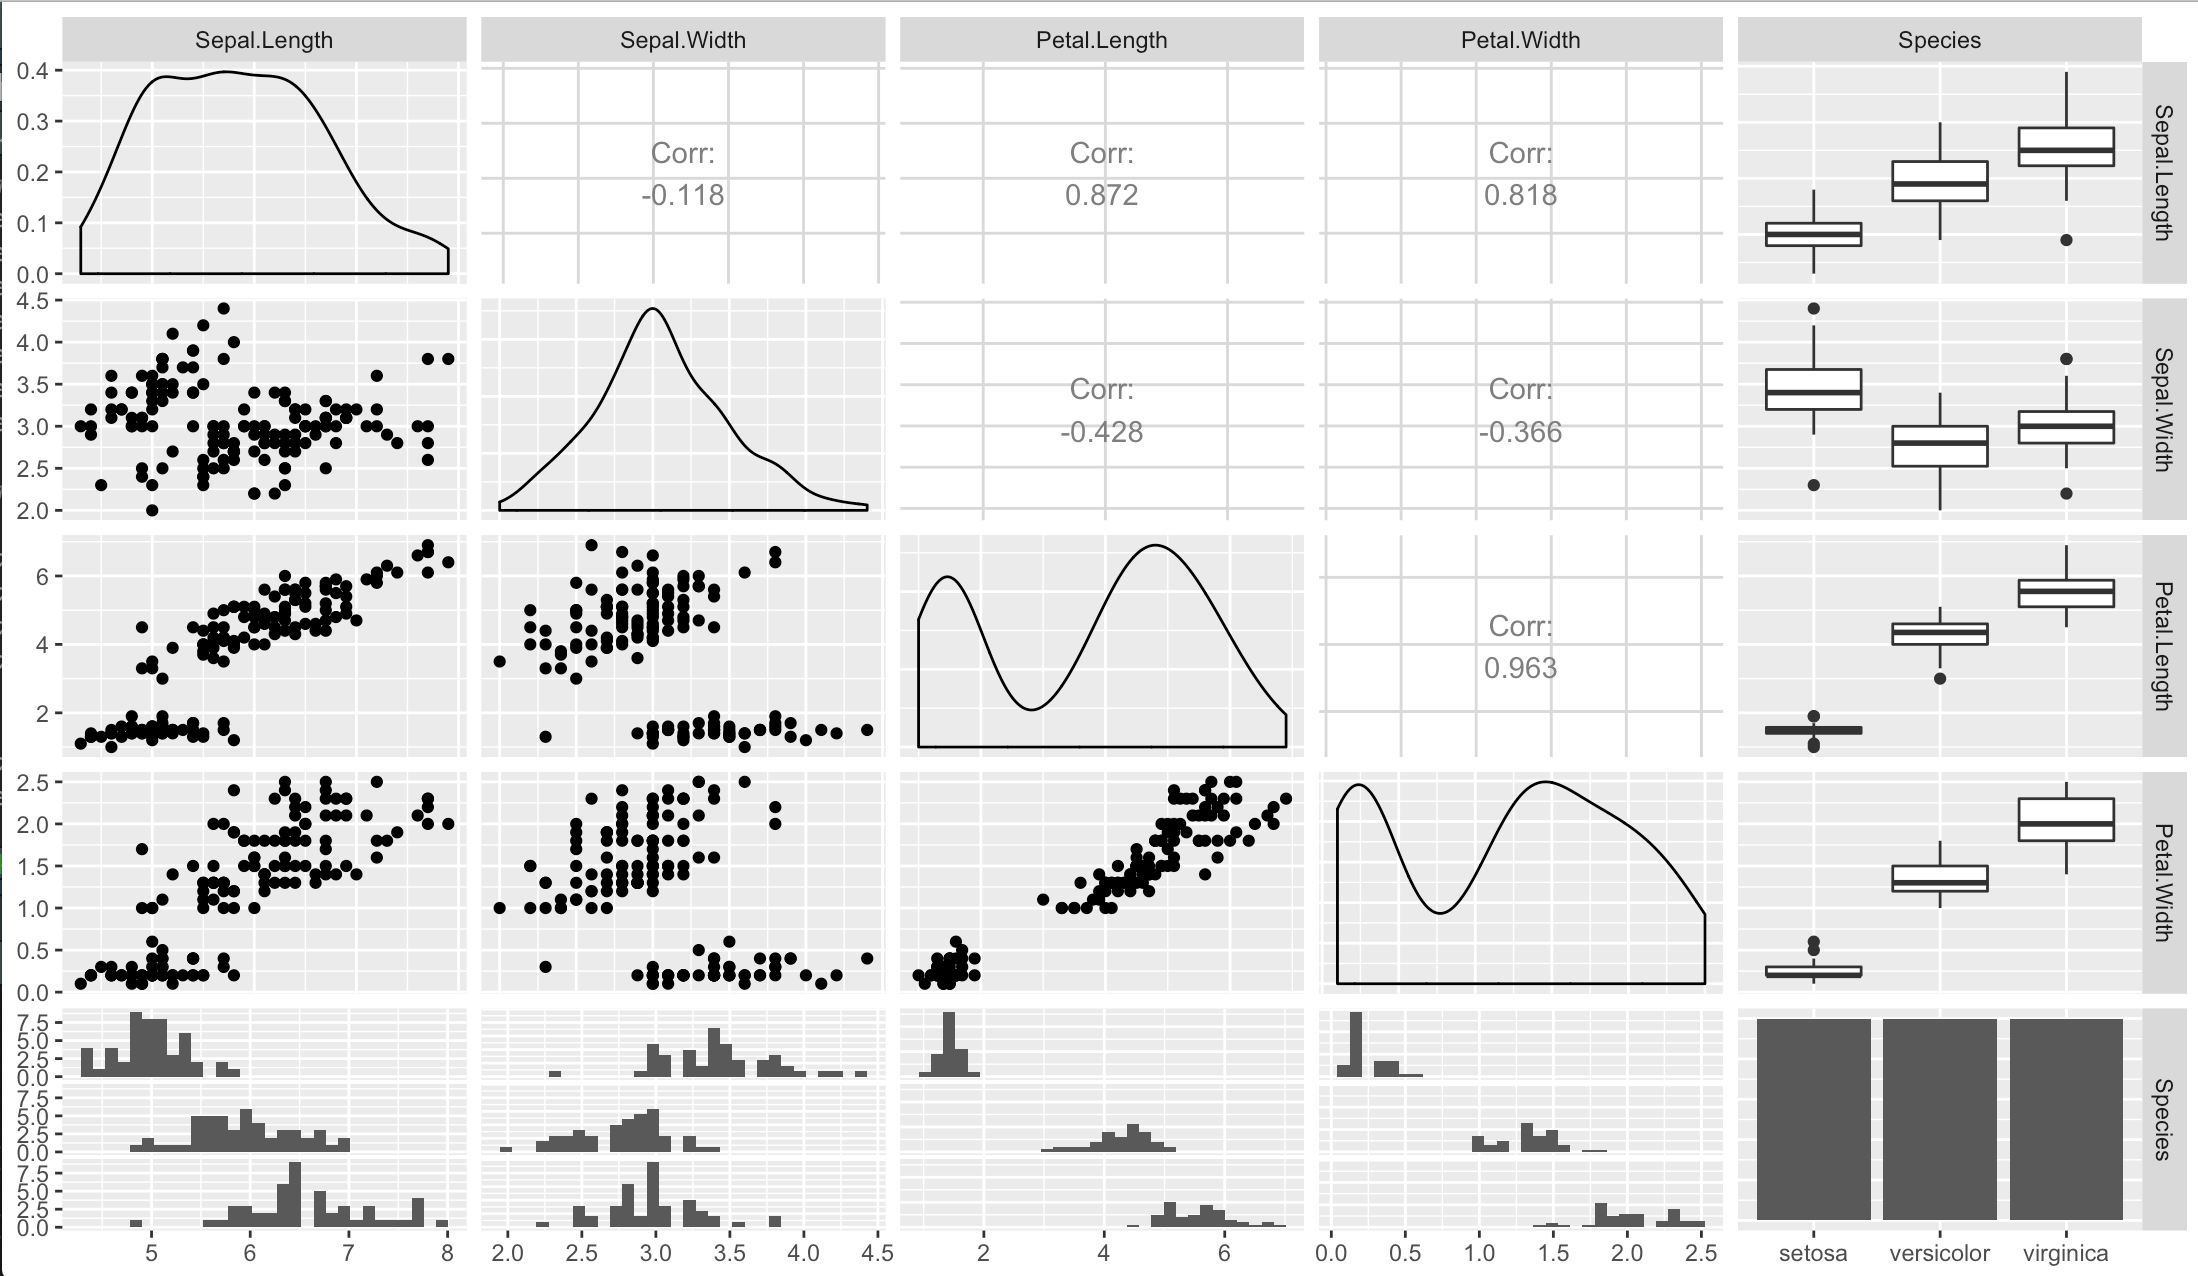
\includegraphics[width=15cm]{Figuras_tfg/R_plot_correlation.png}
  \caption{The GGally package also provides useful tools for this types of problems. Here, the correlation between Petal.Length and Petal.Width is proven to be very high, as the plots from Figure \ref{fig:figure_knn_classifier}}
 \label{fig:figure_knn_classifier_correlation}
\end{figure}

\subsection{Multilayer Perceptron}

The Multilayer Perceptron(MLP) has a similar architecture to that of the Deep Neural Networks. Both of them have input, output and hidden layers as well as having nodes and backpropagation for training. They even need their layers to be activated, as well as support the most common functions used in the autoencoders. Some experts would even label it as a slightly less computationally powerful DNN. \par

It would seem as the main interest into MLPs could be to use them for smaller Autoencoders, but actually they possess a very important feature: it can distinguish and classify data that is not linearly separable.This property can help us qualify and compare different types of classification tasks. And as it is interesting to test multiple algorithms to make the most out of our ET, we can use it together with the rest of the classifiers presented in this Section. It can be specially useful when we pair it with the knn classifier, as we will implement both of them in our project to perform the same tasks. We would expect it to generally perform better on more complex datasets than knn, which suffers when data is more difficult to differentiate. \par

\chapter{Development}
\section{Exploratory Analysis}

Before diving into the application of the Autocoder, we firstly have to take a look into the data that we will be using on our project. We want to use a wide variety of them to test our tool in order to find out if the assesments made on the previous section hold when applied on some of the most commonly datasets used in the industry. When selecting between the huge amounts of information available online, it was in our interest to prioritise them according to a series of qualities. They needed to:
 
\begin{description}
	
\item[$\bullet$] Have different lengths, ranging from easily handable datasets (Iris) to more complex and computationaly harder (MNIST).

\item[$\bullet$] Different classification taks, from binary to categorical.

\item[$\bullet$] Clearly differentiable balancing in the datasets, which will help us understand the potential of our tool.

\end{description}

The following section will help understanding these points and its implications on our task. To do so, a brief description of them and its role on achieving our desired results will be tackled. Descriptions of each dataset will include statistics on their distributions as well as why they were chosen as a viable candidate to fulfill our goal. Mainly we will be relying on simple computations, such as the median, and trying to plot histograms or similar figures to have visible and more user friendly inputs to understand why some steps will be applied on future scripts.\par
 
This task is neccesary if we want to have a hint of the outcome of the processes that will take place on the datasets, as well as to shed a light in the difficulty to adapt our scripts and architectures when moving from one dataset to another one.

 

\subsection{Iris}

The Iris flower dataset is a multivariate data set published in the 1936 paper (The use of multiple measurements in taxonomic problems) by Ronald Fisher. The data itself consists of 50 samples from each of the three species of Iris: Iris setosa, Iris virginica and Iris versicolor. Each of them had four of their characteristics tested: the length and the width of the sepals and petals in centimetres. \par

Based on the distribution of the measurements regarded from the dataset, Fisher's data has been referred to as one of the basic staples of data classification due to the fact that it is divided into two clearly differentiable clusters, one containing Iris setosa and the other one including both virginica and versicolor. Without the labels provided by Fisher, the classifying task becomes more complex. This feature is specially useful to highlight the differences between unsupervised and supervised classification.\newline

\begin{table}[H]
		\caption{R summary method on Iris.}
	\begin{center}
	\label{tab:table_Iris}
		\begin{tabular}{r|c|c|c|c} % <-- Alignments: 1st column left, 2nd middle and 3rd right, with vertical lines in between
			\textbf{Variable name} & \textbf{Sepal Length} & \textbf{Sepal Width} & \textbf{Petal Length} & \textbf{Petal Width}\\
			\hline
			Minimun & 4.30 & 2.00 & 1.00 & 0.10\\
			Median & 5.80 & 3.00 & 4.350 & 1.30\\
			Mean & 5.84 & 3.06 & 3.76 & 1.20\\
			Maximun & 7.90 & 4.40 & 6.90 & 2.50\\
		\end{tabular}
	\end{center}
\end{table}

The table of top contains a summary of the most important statistical features of iris, and by looking at it we can already see that the data is very balanced on every feature as the distance between the Minimun and the Maximun divided by two is approximately the Mean, which also has a close value to the Median. To us, this means that the data is centerred over a certain value, which will allow us to simplify our tasks by doing some type of translation transformation over the data before fitting it through our tools. Regardless, plotting will also help us discern the real difficulty of our classification task.

\begin{figure}[H]
	\centering
	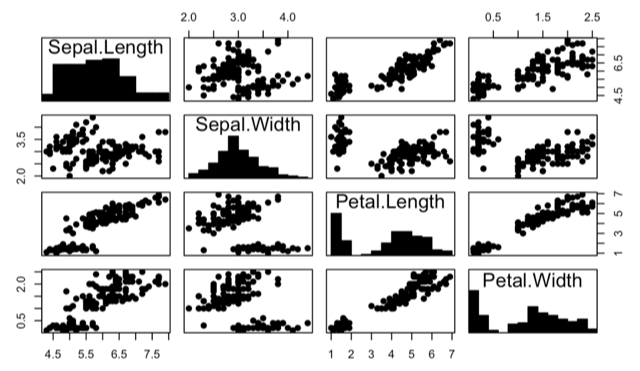
\includegraphics[width=13cm]{Figuras_tfg/Figure_Iris_Histogram}
	\caption{Using the pairs function summary}
	\label{fig:figure_pairs_iris}
\end{figure}

\begin{figure}[H]
\begin{minipage}{.5\textwidth}
        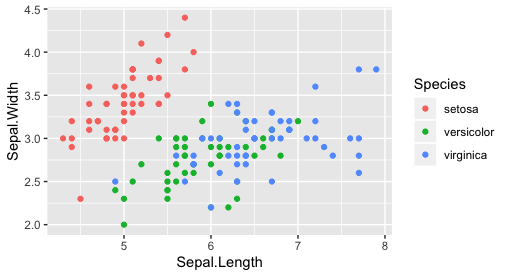
\includegraphics[scale=.54]{Figuras_tfg/R_plot_iris_knn_width_sepal}
 \end{minipage}%
 \begin{minipage}{.5\textwidth}
        \begin{flushright}
               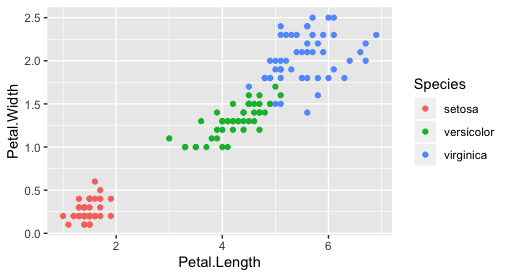
\includegraphics[scale=.54]{Figuras_tfg/R_plot_knn_petal}  
        \end{flushright} 
    \end{minipage}  
  \caption{Plotting of two different features of Iris with respect to the class label. As it can be seen here, depending of how you organise your data you can get more efficient classifiers and clusters. }
 \label{fig:figure_knn_classifier}
\end{figure} 

Taking a look at Figure \ref{fig:figure_pairs_iris}, The histogram on the middle is showing some higher values in different ranges on our data. If we hadn't observed the summary values on the Table \ref{tab:table_Iris} , we could have struggled coming up with the general idea behind the dataset. But sometimes histograms are a little bit more troubling to read into, so plotting Figure \ref{fig:figure_knn_classifier} can help understanding the relationships between classes and their features. For example, the iris dataset would be a good fit for a knn classifier, as its data classes and observations are clearly distinguinshable when using Petal Width and Petal Length rather than when using Sepal Width and Sepal Length. \par

\subsection{MNIST}

The MNIST dataset is a large database of handwritten digits widely used in the data science field both for training and testing. It is mostly used for image processing and it is composed by samples of handwriting taken from the National Institute of Standards and Technology original datasets. It was later normalised to fit into 28x28 pixel images. Every image has a value from 0 to 255 ,which defines the shape and color of the number in the image. Then, the y class contains vectors with a character which can be related to its corresponding pixelised image by a classification method. \par

The database contains 60000 training images and 10000 testing images for $X$ and $Y$. Many different papers (name one) have tried to achieve the lowest error rate on it. Convolutional neural networks manage to get a very low error of around 0.23, although other methods such as support-vector machine get an error of as low as 0.8 too.\par

\begin{figure}[H]
\centering
  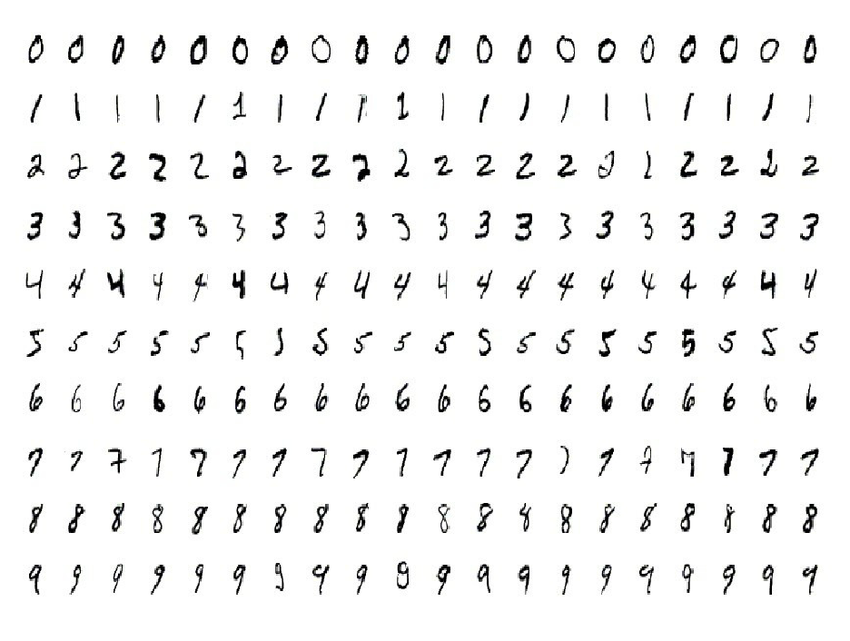
\includegraphics[width=16cm]{Figuras_tfg/Figure_MNIST}
  \caption{Some examples of the images included in the MNIST dataset}
 \label{fig:figure_MNIST}
\end{figure}

\begin{table}[H]
	\caption{R summary method on MNIST.}
	\begin{center}
		\label{tab:table_MNIST}
		\begin{tabular}{r|c|c|c|c} % <-- Alignments: 1st column left, 2nd middle and 3rd right, with vertical lines in between
			\textbf{Variable name} & \textbf{Minimun} & \textbf{Median} & \textbf{Mean} & \textbf{Maximun}\\
			\hline
			X training & 0 & 0 & 33.32 & 255 \\
			X testing  & 0 & 0 & 33.32 & 255 \\
		    Y training & 0 & 4 & 4.454 & 9 \\
		    Y testingg & 0 & 4 & 4.443 & 9 \\
		\end{tabular}
	\end{center}
\end{table}

Using the previously mentioned summary method on the training vectors for $X$ on this particular dataset will not provide us with enough information to estimate the classification task complexity. As we can see from Table \ref{tab:table_MNIST}, we just will know the range of values of every image (already discovered in the definition on the dataset) and the Mean, which only states that out training pixels tend to be white rather than black. In this case, since all of our bits are white or black (255 or 1 in decimal representation), it is on our best interest to try to simply our task by dividing our training and test numbers into binary representations of their types. Achieving it will only mean to transform them into 1s and 0s, and easier representation to handle for our transformation block. \par 

If we instead observe the summary from the $Y$ training data we can see that the dataset is very balanced, as the mean is close to half of the distance between the Minimum and the Maximum. This tells us that we will be able to probably achieve high degrees of accuracy on our classifier, as well as that the Entropy Triangle should also perform a satisfying job when analysing its informational flows.  \par

Our goal when fitting MNIST (located in the tensorflow package) through the autoencoder is to asses its capabilities when using bigger chunks of data and compressing it. Numerous reports and information available online give plethora of information about possible classification methods and its expected outcome in terms of error rates and accuracy. We are not trying to improve their results, we are just mimicking their processes and applying some of their methods so that we can achieve similar results when applying our tools.\par

\subsection{Ionosphere}

Ionosphere represents a set of data collected by a radar in Goose Bay, and later used for data science purposes by the Johns Hopkins University. The antenna had a phased array of 16 high-frequency antennas and used times pulses and pulse numbers for processing. The outputs can be labeled as either "good" or "bad", referring to the fact that a radar signal going through the ionosphere and thus showing no evidence of the existence of an ionosphere was labelled as "bad", and in any other case we would be labelling it as "good". It can be found on the R package mlbench. \newline

\begin{figure}[H]
	\centering
	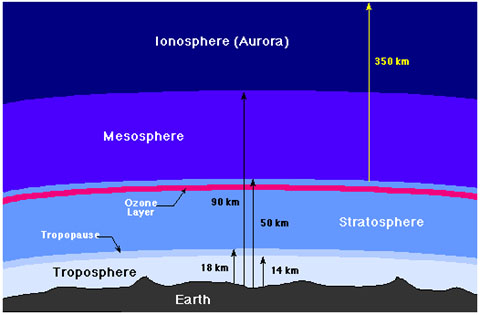
\includegraphics[width=10cm]{Figuras_tfg/Ionosphere}
	\caption{The Ionosphere is one of the main layers composing Earth's atmosphere}
	\label{fig:figure_pairs_iris}
\end{figure}

There are 351 observations from 35 independent variables, with 33 of them being numerical values and 2 of them representing nominal values (one of them defining the class). However, one of the variables included in the dataset can be safely removed since it only represents a constant value (0). Having removed that one it should be remarked that this dataset is not balanced, since we don't posses the same number of "good" or "bad" class labels, and the difference is big enough to potentially affect its transformation and classification.We can expect its performance to be worst than the other two datasets mentioned previously. In the Ionosphere case, we will classify our data using binary decision, as there are only two states available for our labels. \par

Researchers at [Sigillito, V. G., Wing, S. P., Hutton, L. V., \& Baker, K. B. (1989). Classification of radar returns from the ionosphere using neural networks. Johns Hopkins APL Technical Digest, 10, 262-266.] have found very high acurracies when using non-linear perceptrons on this dataset, but to do so they had to use the quantities of "good" and "bad" observations, which would not fit our needs of information. Although it can be easily inferred that we are going to get some degenerated results when compared with other papers, it seems like an appropriate choice to check the performance of our tool. \par 

\chapter{Results}

In this section we will be presenting the results regarded from the different experiments performed over the datasets using the methods previously introduced. All the experiments will have different sets of requirements and levels of complexity, which will help us discern the capabilities of the tools involved. To be able to do so, we have to establish the same structures of tests.

\begin{figure}[H]
\begin{subfigure}{1\linewidth}  
 \centering
  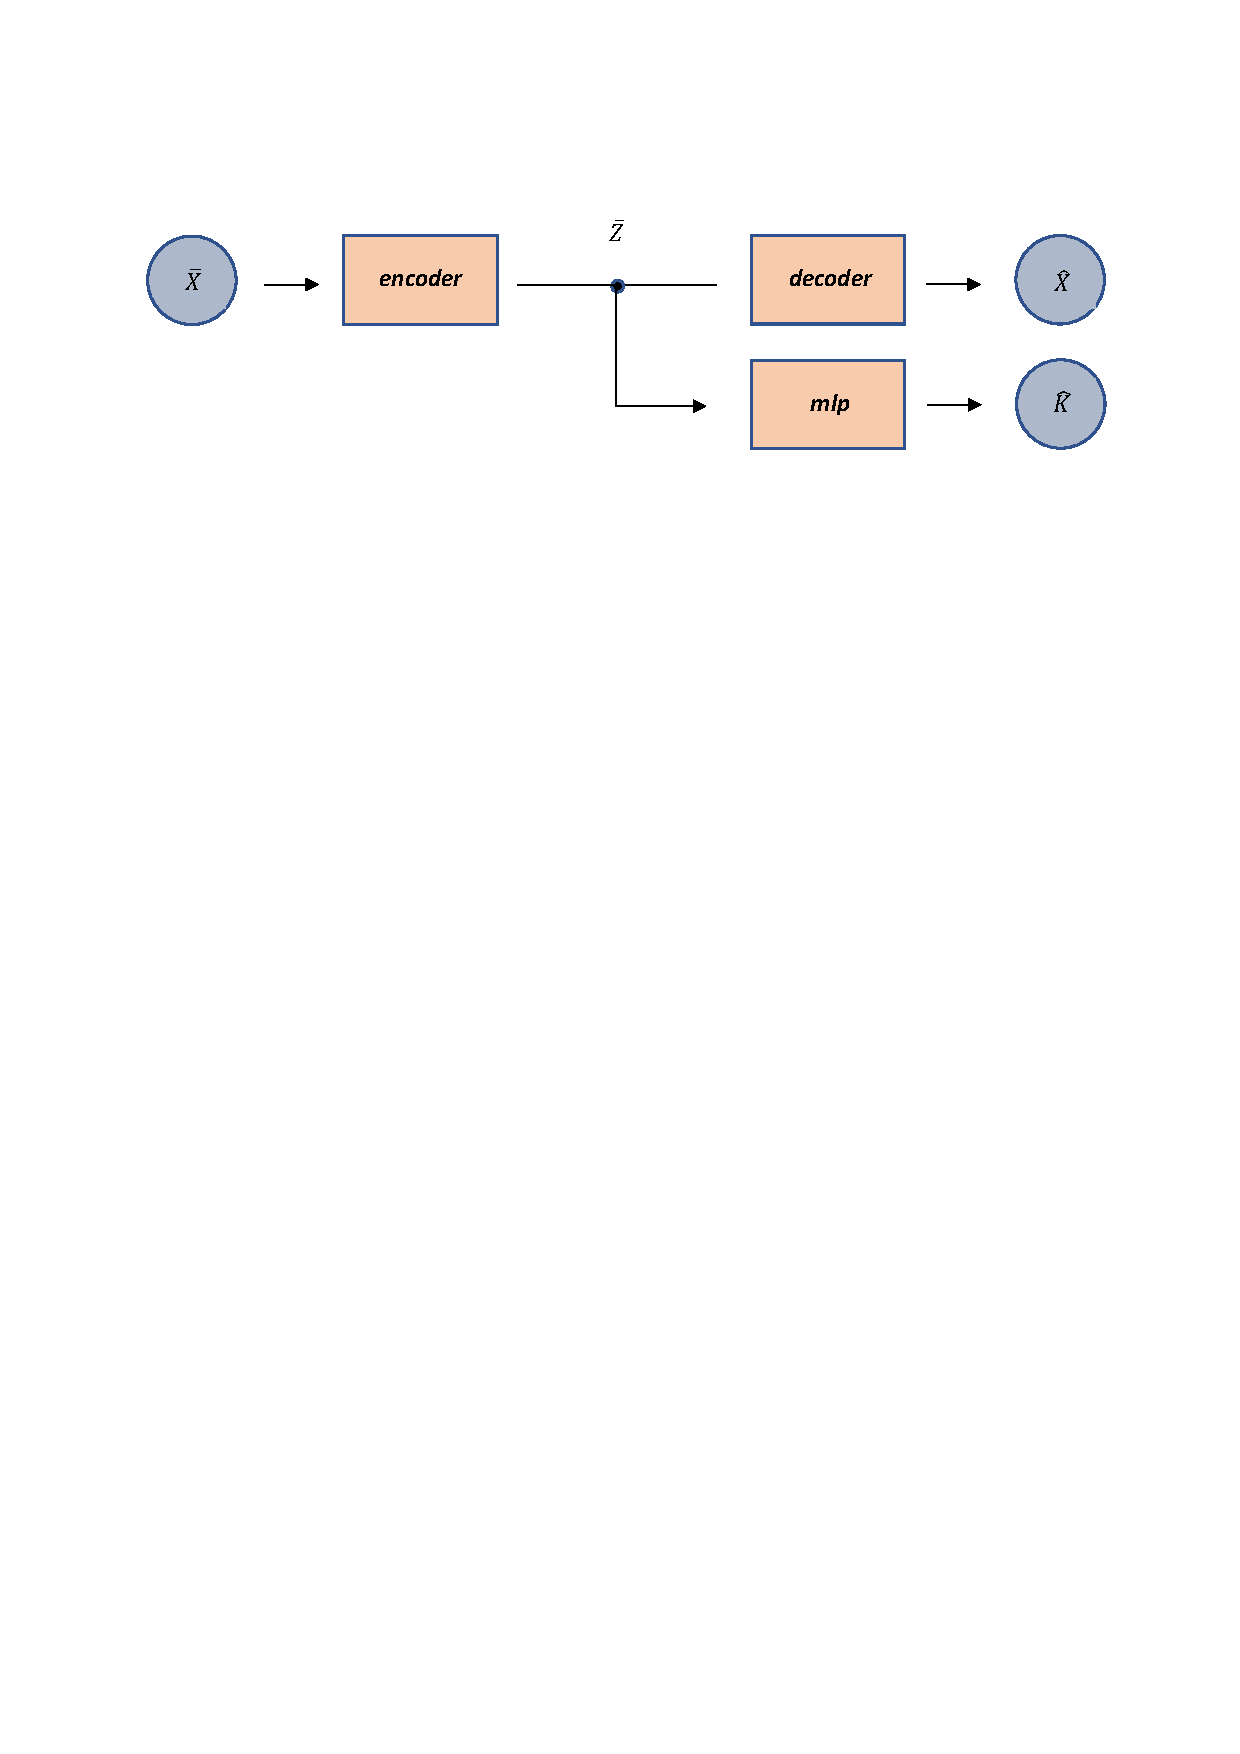
\includegraphics[width=\linewidth]{Figuras_tfg/Diagram_auto_mlp}
  \caption{Autoencoder and MLP.}
  \label{fig:FigA_Autoencoder_MLP} 
\end{subfigure}

\begin{subfigure}{0.98\linewidth} 
  \centering
  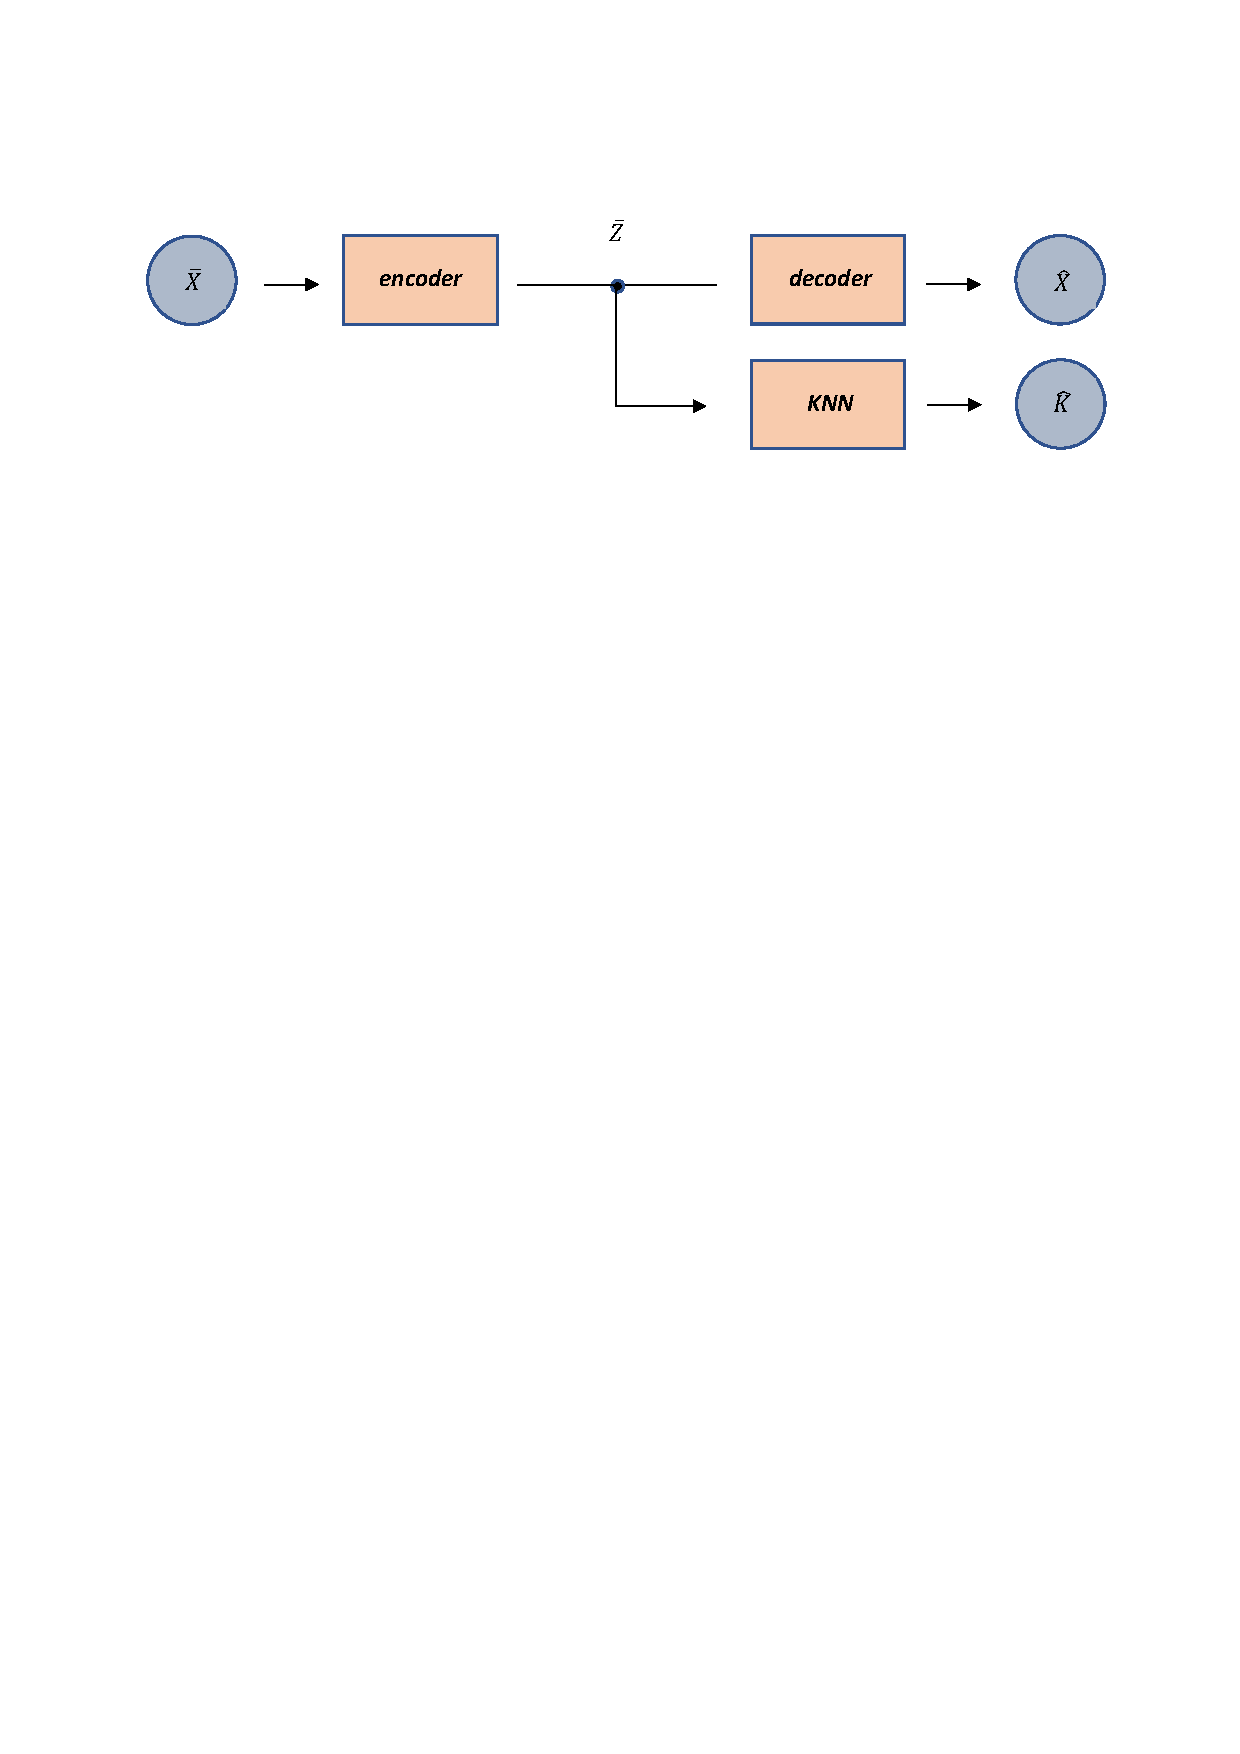
\includegraphics[width=\linewidth]{Figuras_tfg/Diagram_auto_KNN}
  \caption{Autoencoder and KNN.}
  \label{fig:FigB_Autoencoder_KNN} 
\end{subfigure}
  \caption{Structure of the Autoencoder and it's classifiers}
 \label{fig:Autoencoder_architecture}
\end{figure}

As seen in Figure \ref{fig:Autoencoder_architecture}, we will use the representation of our encoded data $\hat{Z}$ as the input for both the KNN and the MLP classifiers.


\begin{figure}[H]
\begin{subfigure}{1\linewidth}  
 \centering
  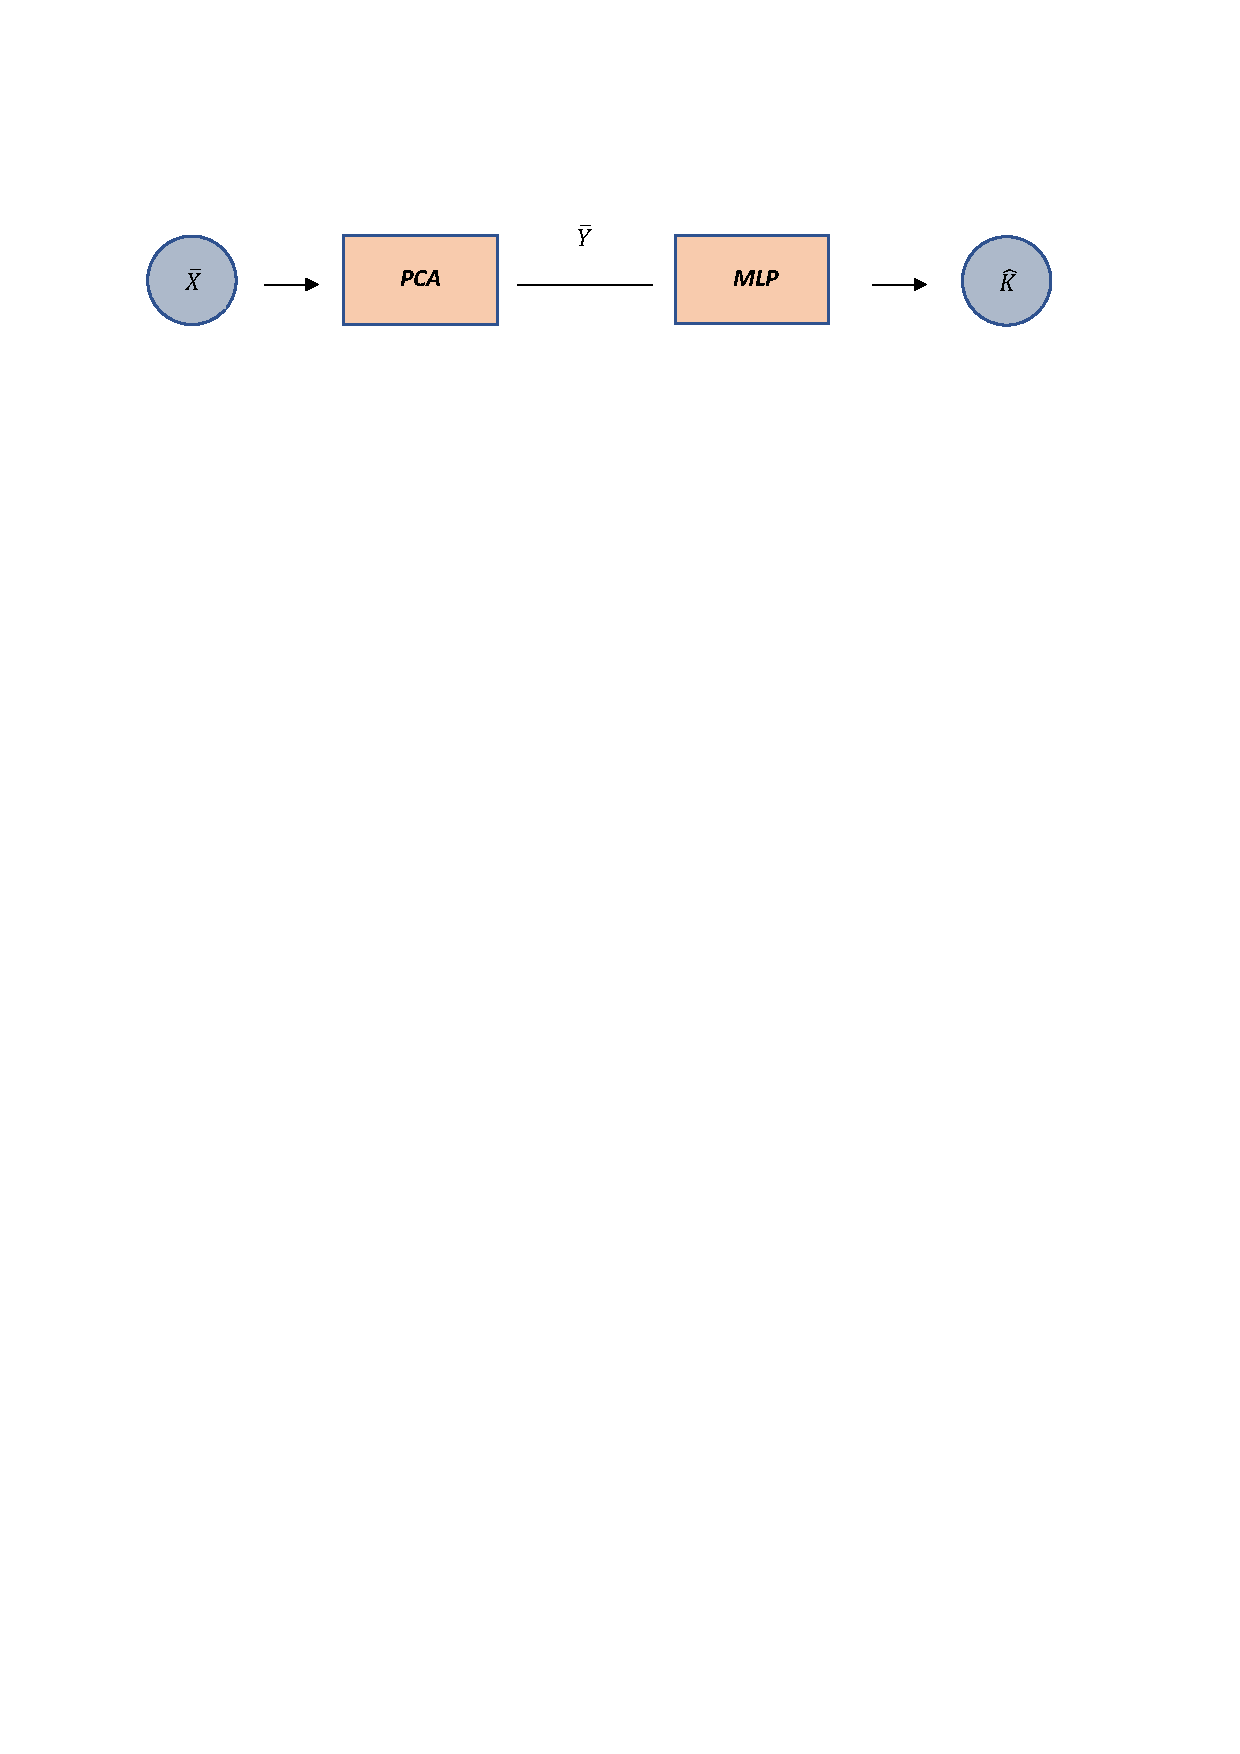
\includegraphics[width=\linewidth]{Figuras_tfg/Diagram_pca_mlp}
  \caption{PCA and MLP.}
  \label{fig:FigA_PCA_MLP} 
\end{subfigure}

\begin{subfigure}{1\linewidth} 
  \centering
  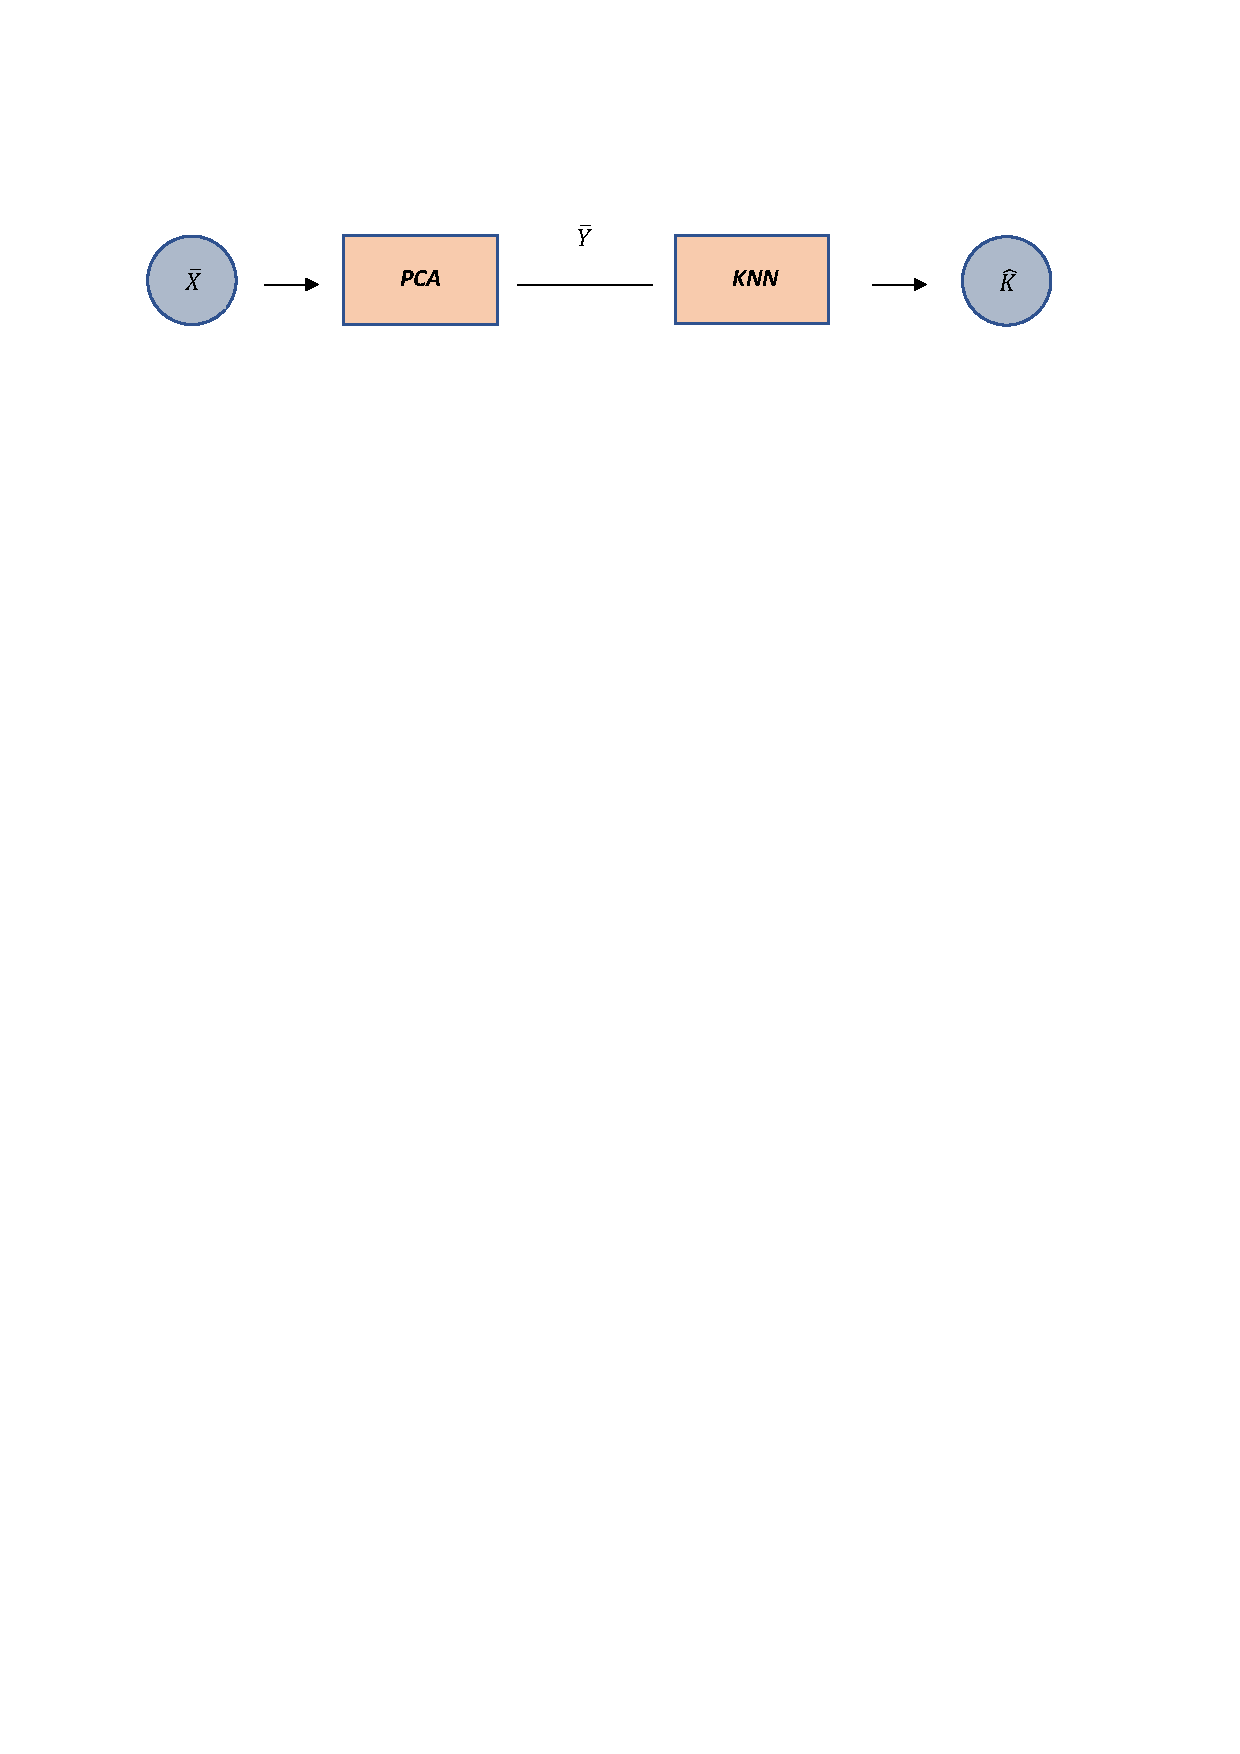
\includegraphics[width=\linewidth]{Figuras_tfg/Diagram_pca_KNN}
  \caption{PCA and KNN.}
  \label{fig:FigB_PCA_KNN} 
\end{subfigure}
  \caption{Structure of the PCA and it's classifiers}
 \label{fig:PCA_architecture}
\end{figure}

If we compare both the structures presented here, we can see in the images in Figure \ref{fig:PCA_architecture} that we will be using the output from the PCA as the input of the classifiers, as well as that we will have the same classifiers used in both architectures, with the aim to be able to compare their results.\par

As we are also concern about the reliability of them too, we will be including another technique to try to validate our results as much as possible: K-Fold validation. \par

K-Fold is a method which is based on dividing a dataset into K folds, each one of them not sharing the same elements on their observations. We are interested into really asserting how each of the Folds of our datasets performs by fitting them through the structures presented in both Figure \ref{fig:Autoencoder_architecture} and \ref{fig:PCA_architecture}. Once we have each one of them complete the full training process, we will analyse the output plus the summation of the overall results. We expect our Folds to provide us with similar data and results in our plots when we use balanced datasets. However, if we have unbalanced datasets we expect to see more inconsistency through them.\par

At the end of each section, the overall performance of each dataset will be tested with the Entropy Triangle, which will be used to compare the entropy between the data of each Fold generated at the beginning of the process and the output of the classifier.

\section{Iris Dataset}
\subsection{Data Preparation}

In order to train the data through the Autoencoder, we will firstly have to transform it into an easier shape which will reduce the difficulty and length of our task. Normally, Deep Neural Networks will do a good job as long as the data has a reasonable scalability, so applying a normalisation to our data is not mandatory. However, it is easier for us to use a simple pre-processing in our data, which given that the observations from the variables have different ranges of values will help us reduce the training time of our Autoencoder.

Although as we can see from Figure \ref{ig:figure_pairs_iris} and Table \ref{tab:table_Iris}, some of its features are closer to what it could be referred as a Normal distribution, specially Sepal Length and Sepal Width. Other's, such as Petal Length, are a little bit off and far away from that description. To be able to fix those disparities, we will apply a Box-Cox transformation, which consist basically of applying the following equation on your data:

\begin{equation}
\label{eq:box-cox}
 {y(\lambda)=} \left\{
 \begin{aligned}
        \frac{y^{\lambda} - 1}{\lambda} ,  if \  \lambda \neq 0\\
        {\log y}, if \ \lambda = 0
       \end{aligned}
 \right\}
 \end{equation} 
\newline

Where $\lambda$ is an exponent which value inside the range $[-5,5]$. The Box-Cox method will automatically assign the value of lambda that fits your dataset the most. This value is selected simply by looking for the optimum value by fitting the equation \ref{eq:box-cox} . \par

Once we apply this function, we can start to see the results on our newly created data by checking its pairs function again:

\begin{figure}[H]
	\centering
	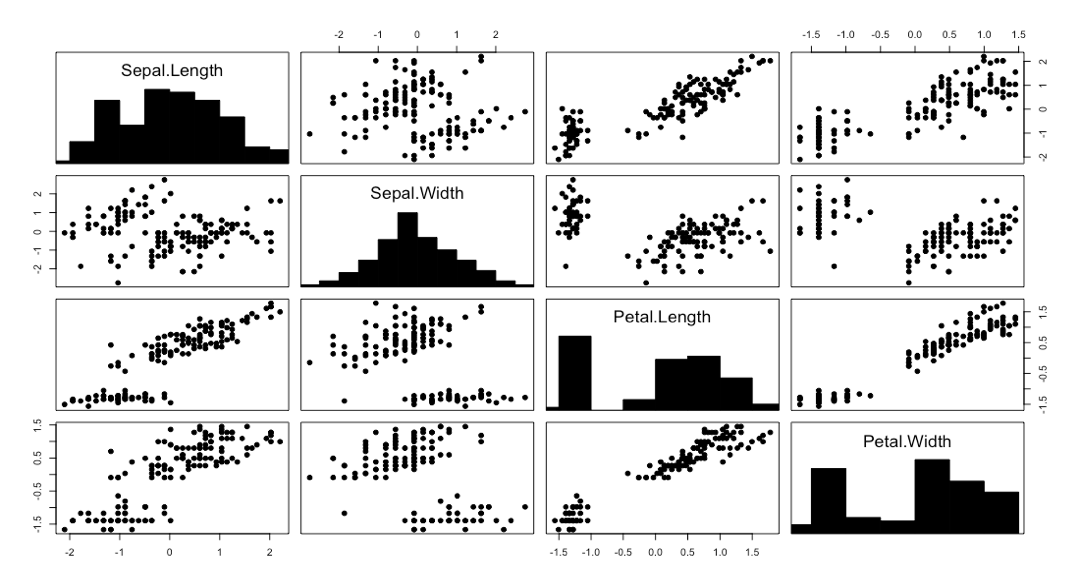
\includegraphics[width=17cm]{Figuras_tfg/Figure_Boxcox}
	\caption{Using the pairs function on Iris Boxcox}
	\label{fig:figure_pairs_iris}
\end{figure}

Which has an histogram slightly different to the one presented on Figure \ref{fig:figure_pairs_iris}, but we can really see the new features of our transformation if we use use the summary function and compare its results with respect to the ones obtained before on Table \ref{tab:table_Iris}
\newline

\begin{table}[H]
		\caption{R summary method on Iris Box Cox.}
	\begin{center}
	\label{tab:table_Iris_Boxcox}
		\begin{tabular}{r|c|c|c|c} % <-- Alignments: 1st column left, 2nd middle and 3rd right, with vertical lines in between
			\textbf{Variable name} & \textbf{Sepal Length} & \textbf{Sepal Width} & \textbf{Petal Length} & \textbf{Petal Width}\\
			\hline
			Minimun & -2.10 & -2.75 & -1.56 & -1.66\\
			Median & 0.02 & -0.08 & 0.33 & 0.27\\
			Mean & 0.00 & 0.00 & 0.00 & 0.00\\
			Maximun & 2.20 & 2.75 & 1.78 & 1.45\\
		\end{tabular}
	\end{center}
\end{table}

By looking at the Table on top, it can be seen that as expected the Mean of our distribution switched from it's previous value to 0, essentially telling us that the transformation has been successful. It is also important to point out that although the values of the vector that are in our dataset are different, we still hold the same proportions and plots of the observations, which means that the general information that each of our variables contained its still there. We just shaped it differently so that it is easier for us to work and perform operations with them.

\subsection{The Autoencoder}

For the Iris dataset, we will use a simple Autoencoder, with just a few layers, that should be enough to complete the training required. As our given dataset doesn't contain a lot of observations, this approach to the Autocoder has the aim to show an example of use. That is why , if we take into account that we only have for variables to compress, we can see that the maximum compression we can achieve is a 25 percent of the original size. But, in order to be sure we have a working architecture, I will be using just a 75 percent compression in the middle layer. On the other hand, our model will have a data expansion of about 400 percent, so that we are able to do a real compression in each of the subsequent layers. \par

\begin{figure}[H]
	\centering
	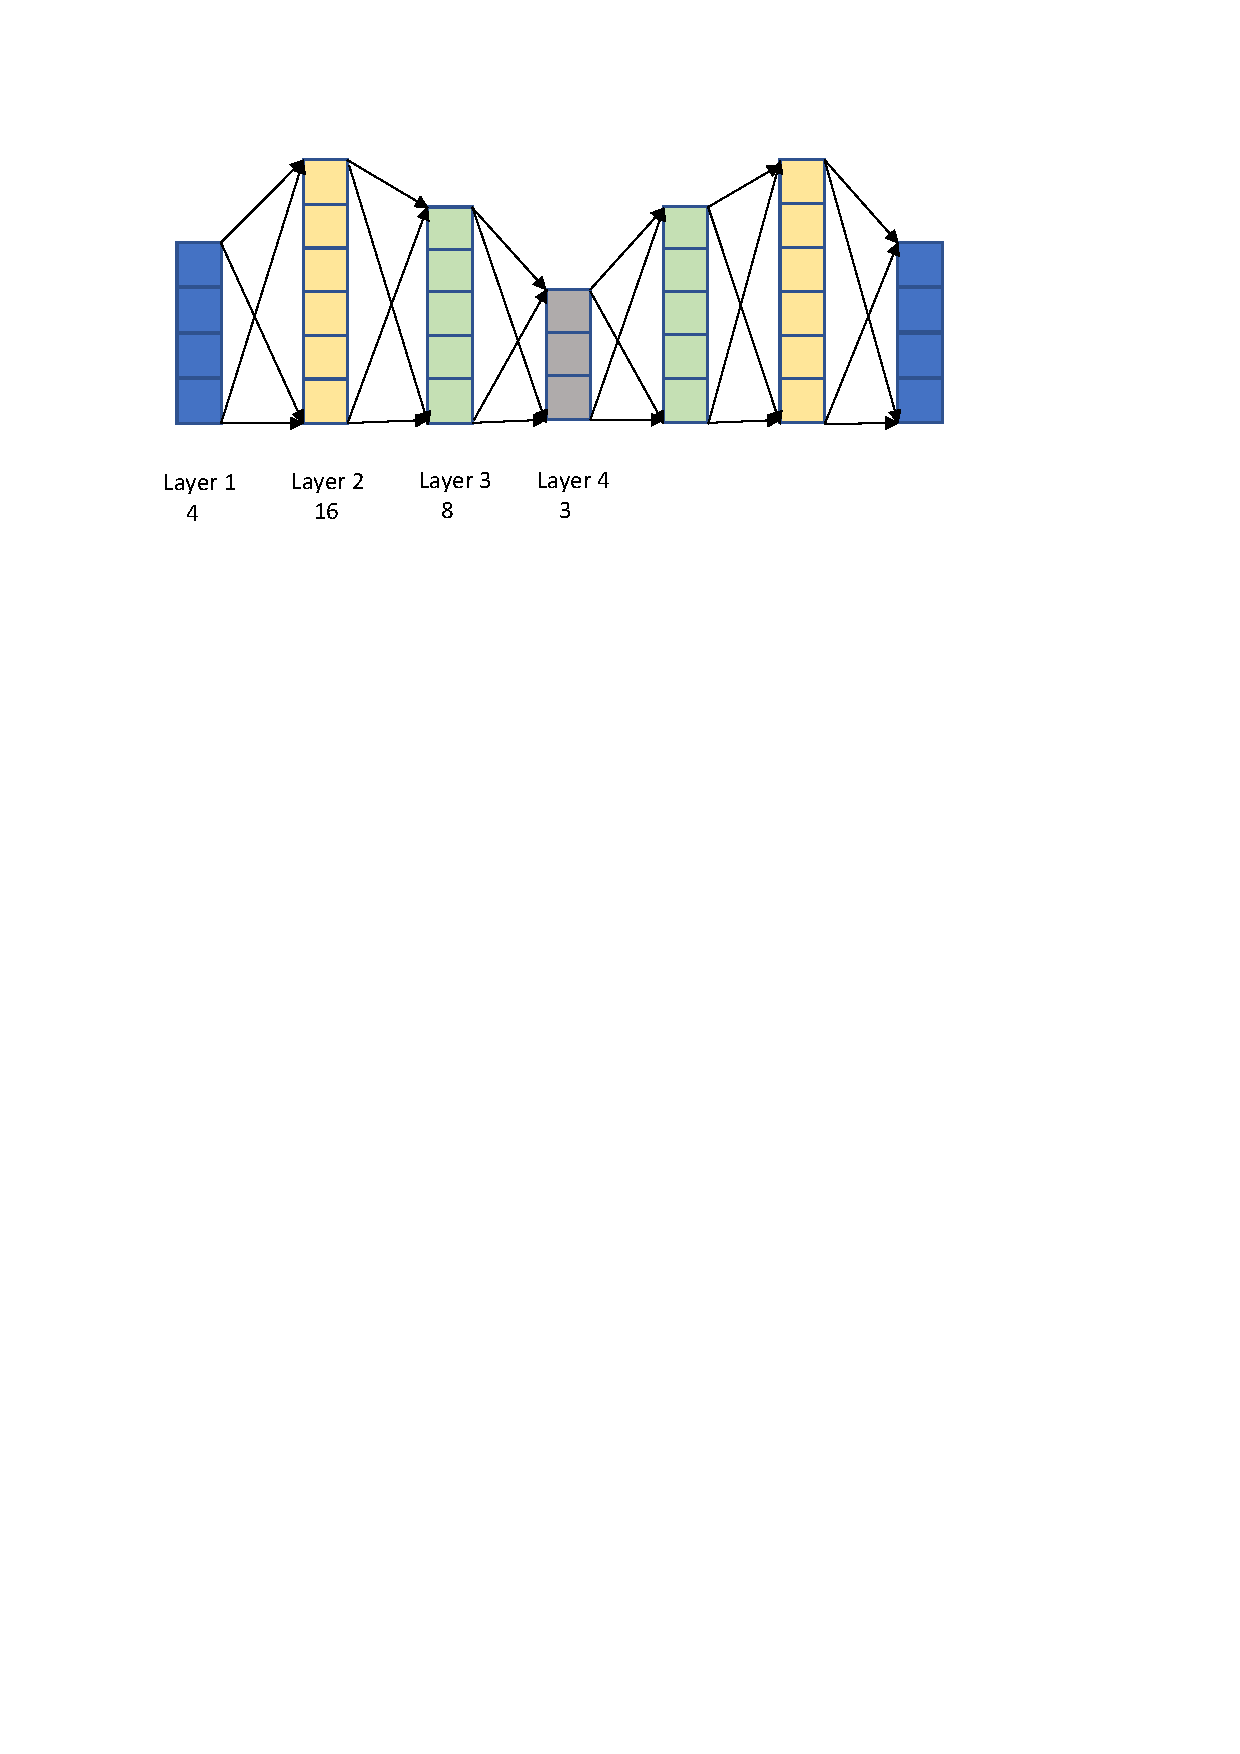
\includegraphics[width=17cm]{Figuras_tfg/Autoencoder_Results}
	\caption{Architecture of the Autoencoder in Iris}
	\label{fig:figure_autoencoder_Iris}
\end{figure}

On Figure \ref{fig:figure_autoencoder_Iris}, each of the layers has the size assigned below it. But before choosing the compilation method we are going to use for the Autoencoder, we have to choose the activation functions for each layer. In this case, we decided that the Relu function would be used (for all the layers of the Autoencoder except the last one), where we will use a sigmoid function. We decided to use this setup because the Relu function does a good job at selecting the informational qualities of each component while at the same time keeping the training time of the architecture very low due to the simplicity of its definition, while the sigmoid function is more complex and thus seems to be suited for the last layers and to finalise the transferring of information. \par

The last thing to take into account is the compilation of the whole structure created with the previously mentioned Autoencoder. Here, we will have to choose between the wide range of available options on the keras package, to try to maximise the performance and optimisation of our model. To do so, we have to first rule out all the loss functions that don't apply to our task. For example, although used in a lot of DNNs, the categorical functions don't fit our criteria since we are not performing a classification task here. Moreover, our range of data is not between 0 and 1, which would make this even a worst choice. For us, since we also are trying to predict the output data using some training data, we can assume we have a (regression problem) in our hands.\par

Having stablished that, we have a narrower set of possible choices to make. Between all of the available, we decided to use the (Mean Squared Error function). The MSE is calculated as the average of the squared differences between the predicted and the original values. This means that the bigger the difference them, the more punitive this metric is for our model. This works great for the intent of our experiments, since we want our model to be able to get very accurate predictions from the compressed version of our data. \par

Finally, we also need to decide on our optimiser for our compilation. Here we decided to narrow our options to chose only between the Adam and the Adadelta options. Finally, it was seen that the Adam optimiser was achieving the same level of losses as the Adadelta, while needing less epochs. Due to the amount of passes that we have to do through the Autoencoder, it is useful for us to get reliable data in the shortest time possible, so it was finally implemented using Adam.This decision would allow us to help mitigate the problem of time, which can be quite demanding when dealing with multiple transformations and neural networks.

\subsection{The Classifiers}

\subsubsection{Knn on PCA and Autoencoder}
Once we have obtained the output of our Autoencoder, we have a resulting data frame with the same number of observations but a reduced number of variables, which in the case of the Iris Autoencoder will be three, making our resulting matrix to have a shape of $120\times3$. It also must be notest that the process is the same for both the output of the Autoencoder and the PCA.\par

The matrices resulting from this compression process may not have all of their columns or rows with a value different from 0. This does not pose a threat to our training, since none of the methods chosen for our training will drop our results. In the case of the Knn  we will get some Warnings, but as we will see later it won't affect the result of the process. \par


\begin{figure}[H]
	\centering
	\includegraphics[width=15cm]{Figuras_tfg/Knn_example}
	\caption{Knn example on Iris}
	\label{fig:figure_Knn_Iris}
\end{figure}

The function that we decided to use for our Knn training was provided in the train method in the caret package. It only requires you to specify the training data, labelled as x, the labels to be trained with, named as y, and the method, which is a simple Knn classifier. Once provided, the function will start to train your model. \par


Once the model has finished training, we will use the model generated with our values to predict the labels of our model and compare it to the labels we used to train it on the first place. Once we have calculated that, we will use the confusionMatrix function to asses the accuracy of our predictions when compared to our original labels. A Confusion Matrix is a table with the same number of columns and rows as your class labels, being the only difference that the diagonal represents the predictions from your model and the class labels that matched, while anything outside of it accounts for the number of missed predictions with respect to the class. In this case, this method will provide us with a $3\times3$ matrix which we then can feed to the jentropies method. \par


\begin{figure}[H]
	\centering
	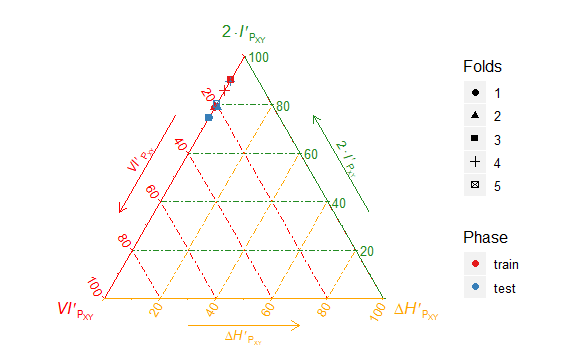
\includegraphics[width=1.2\linewidth]{Figuras_tfg/ET_knn_iris_auto}
	\caption{Entropy Triangle in Knn in Iris using the Autoencoder}
	\label{fig:figure_Knn_Iris_ET_Auto}
\end{figure}

\begin{figure}[H]
	\centering
	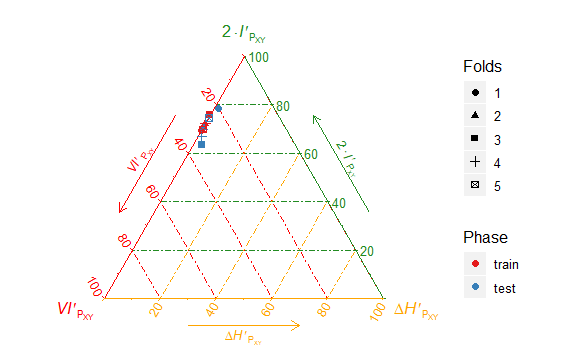
\includegraphics[width=1.2\linewidth]{Figuras_tfg/ET_knn_iris_pca}
	\caption{Entropy Triangle in Knn in Iris using the PCA}
	\label{fig:figure_Knn_Iris_ET_PCA}
\end{figure}

This method will provide us with metrics that then can be used together with the ggmetern method to get a coordinateS inside de Entropy Triangle, which can be seen on both Figure \ref{fig:figure_Knn_Iris_ET_Auto} and \ref{fig:figure_Knn_Iris_ET_PCA}. Given that we are using a K-Folds validation with a value of $K = 5$, we are plotting 5 coordinates for our test and train variables, just to see how well our model performed.\newline

From the Knn on the Autoencoder as seen on Figure \ref{fig:figure_Knn_Iris_ET_Auto}, we can see that the coordinates from the training and testing are close to each other spatially, which means that we have done a good job overall at training our model. Some of the folds seem to have performed worse that the other, but that can just be that the other performed extremely well with their predictions. Specially the First fold seems to provide the best results, as we are getting a perfect classification as well as the optimum information flow on our Entropy Triangle. To completely be able to asses it's quality, we have to see the overall values of the total Confusion Matrix of the testing phase.\par

On the other hand, the PCA on Figure \ref{fig:figure_Knn_Iris_ET_PCA} has a very centralised amount of values. The majority of the phases from the folds seems to be placed around the same area of the Entropy Triangle. No fold has over-performed the others in a greatly manner, which tells us that the results are consistent all throughout the training, which is not the same case as in the Autoencoder case, where the results are more spread. \par

\begin{figure}[H]
	\centering
	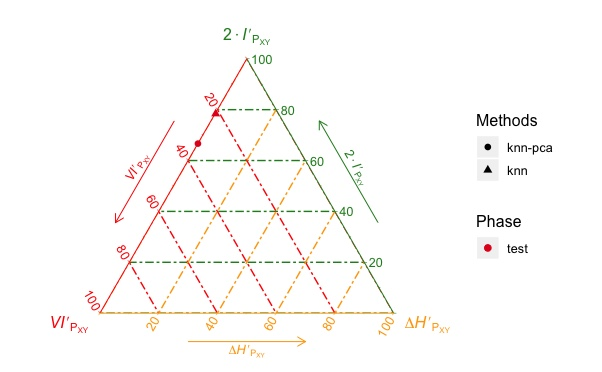
\includegraphics[width=1.2\linewidth]{Figuras_tfg/Total_ET_Knn_Iris}
	\caption{Entropy Triangle in Knn in Iris with the testing results}
	\label{fig:figure_Knn_Iris_ET_PCA_Auto}
\end{figure}

Although the pca has more consistent and less spread results, we can see in Figure \ref{fig:figure_Knn_Iris_ET_PCA_Auto} that the Autoencoder has done an overall better job at providing information for the knn for the classification. Both of them are placed on the side of Triangle $VI_{P_{XY}}$ that accounts for the transference of information, but the Autoencoder is providing a better representation of the data that is allowing the knn to do a better job overall. \par

We can therefore conclude that, in the case of the classification using the  knn on both the PCA and the Autoencoder, we have found the latter to do a better job than the first one informationally speaking, thus leaving us with the assumption that it is the preferred solution for the Iris dataset.

\subsubsection{	MLP on PCA and Autoencoder}

Before fitting the data through a MLP, we have to specify the structure that we are implementing on our Neural Network. Seeing that the PCA and the Autoencoder both predict different lengths for our target training matrices, we have to take into account that the input shape will differ. \par

Once we know that, we can start looking at our structure. Since we are dealing again with a small number of variables, a simple approach will be to divide our MLP into 4 layers. Firstly, we place an input layer with the size of our data, either a $3\times120$ in the Autoencoder or a $4\times120$ in the PCA. Secondly, we can place an expansion layer of size 5, followed by the first compression layer of 4, which is connected to the last one which will be the output of our architecture. \par

\begin{figure}[H]
	
	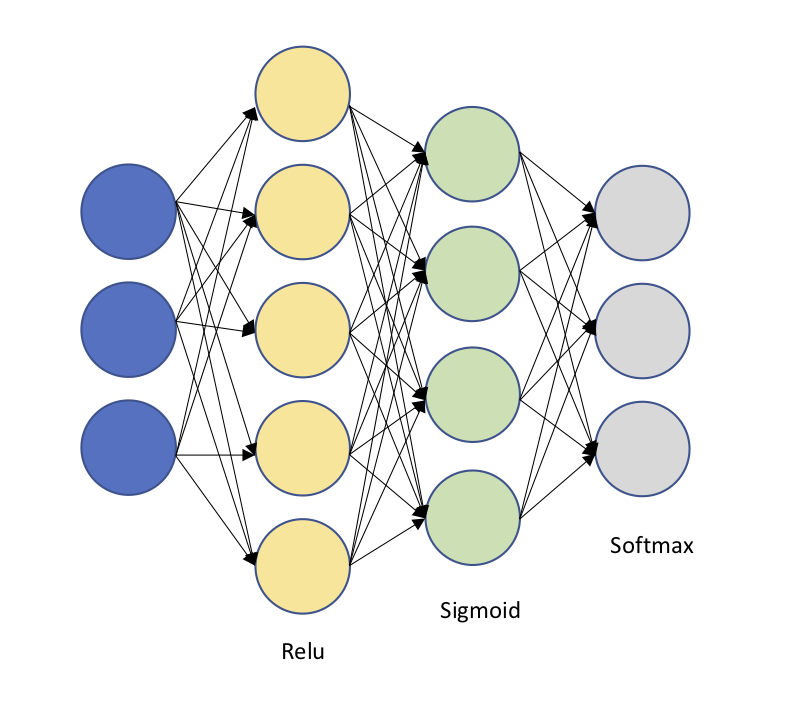
\includegraphics[width=0.8\linewidth]{Figuras_tfg/Example_MLP_Auto.png}
	\caption{MLP architecture in Iris for the Autoencoder}
	\label{fig:figure_MLP_Iris_Autoencoder}
\end{figure}

After figuring out the structure, we now have to decide which activation function would fit the best for each layer. As in the Autoencoder, the first layer will be a Relu, the second one acquires the role of the Sigmoid and finally, as the MLP is a classifier, we have to place a softmax activation function at the end. We want the output of our Autoencoder to be a decision and the softmax is the chosen solution, as we will get our output variables to have an added value equal to 1, being the greater one the label predicted. \par

\begin{figure}[H]
	
	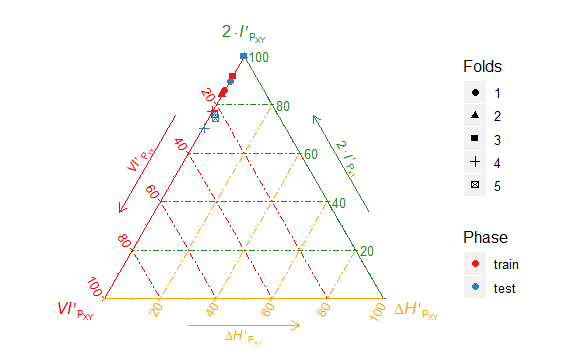
\includegraphics[width=1\linewidth]{Figuras_tfg/ET_Iris_Auto_Mlp}
	\caption{MLP Entropy Triangle in Iris for the Autoencoder}
	\label{fig:figure_ET_MLP_Iris_Autoencoder}
\end{figure}

\begin{figure}[H]
	
	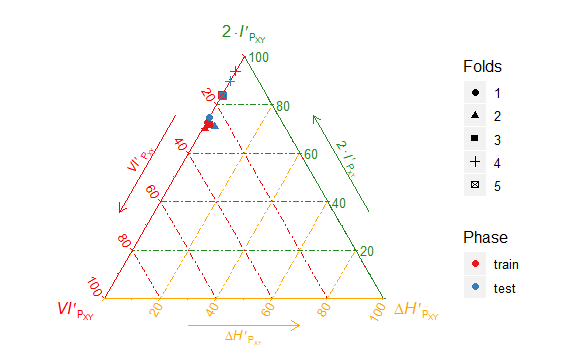
\includegraphics[width=1\linewidth]{Figuras_tfg/ET_Iris_Pca_Mlp}
	\caption{MLP Entropy Triangle in Iris for the Pca}
	\label{fig:figure_ET_MLP_Iris_Pca}
\end{figure}

From Figure \ref{fig:figure_ET_MLP_Iris_Pca} has produced again spatially closed coordinates, which tell us that the folds have been very consistent at training our model. The fourth fold seems to have given slightly worse results, but overall the mlp has generated values that are consistent with our prediction that it would work well with Iris. We can also see that most of the values are grouped on the diagonal of the $VI_{P_{XY}}$, which tells us that our folds have been correctly balanced. \par

On the other side, we have Figure \ref{fig:figure_ET_MLP_Iris_Autoencoder} which seems to have slightly better results overall. We can see the same behaviour on the fourth Fold as before, which tells us that the mlp may have struggled on both cases to train that fold. All of the test folds are close spatially and in the previously mentioned $VI_{P_{XY}}$ diagonal as well as placed very highly on the Entropy Triangle, which tells us that the mlp is being able to classify efficiently. \par
 
 
\begin{figure}[H]
	
	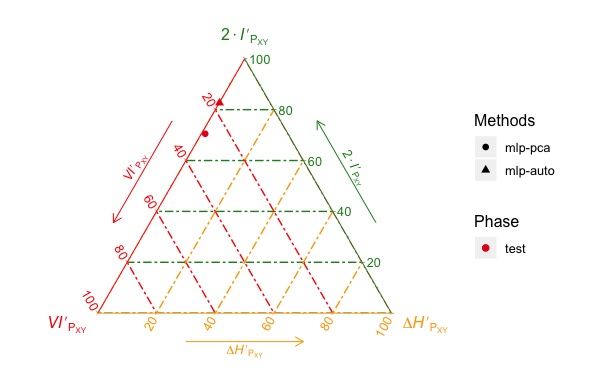
\includegraphics[width=1\linewidth]{Figuras_tfg/ET_Total_Iris_Mlp}
	\caption{MLP Entropy Triangle total testing result}
	\label{fig:figure_ET_Total_MLP_Iris}
\end{figure}

As in the previous cases, we finally have to look at the overall performance of the mlp. In this case, it can be seen that Figure \ref{fig:figure_ET_Total_MLP_Iris} shows a clear advantage of the Autoencoder for the same task. Moreover, if we compare both the results from the Knn and the MLP, we the MLP has the best results for the classification task. On the other hand, we are not seeing a big difference in the performance of the MLP with respect to the KNN, but that may also be because of the simplicity of the Iris dataset.

\section{Ionosphere Dataset}
\subsection{Data Preparation}

The only pre-proccessing done for Ionosphere was explained in the previous section referred to the the datasets. No Box-Cox or other method was found to improve the performance on this particular case. We will only get rid of the column with no variance, which as mentioned before was a column with a constant value of 0 all throughout the set. As explained before, we expect this dataset to show more unbalancing in its results.

\subsection{The Autoencoder}

Ionosphere has more variables that Iris, but it is still a small Autoencoder compared to the structure that we are using for MNIST. The structure that we decided to implement transforms the data provided by the package into 8 observations. We again are using an Autoencoder with the same amount layers structured as:  \newline

\begin{table}[H]
		\caption{Ionosphere Autoencoder layers of the encoder.}
	\begin{center}
	\label{tab:table_Ionosphere_auto_encoder}
		\begin{tabular}{c|c|c} % <-- Alignments: 1st column left, 2nd middle and 3rd right, with vertical lines in between
			\textbf{Layer Number} & \textbf{Size} & \textbf{Activation Function} \\
			\hline
			First & 33 & None\\
			Second & 50 & Relu\\
			Third & 20 & Relu\\
			Fourth or Middle & 8 & Relu\\
		\end{tabular}
	\end{center}
\end{table}

\begin{table}[H]
	\caption{Ionosphere Autoencoder layers of the decoder.}
	\begin{center}
	\label{tab:table_Ionosphere_auto_decoder}
		\begin{tabular}{c|c|c} % <-- Alignments: 1st column left, 2nd middle and 3rd right, with vertical lines in between
			\textbf{Layer Number} & \textbf{Size} & \textbf{Activation Function} \\
			\hline
			Middle or First & 8 & Relu\\
			Second & 20 & Relu\\
			Third & 50 & Relu\\
			Fourth or Output & 33 & Sigmoid\\
		\end{tabular}
	\end{center}
\end{table}

As seen of both Table \ref{tab:table_Ionosphere_auto_encoder} and Table \ref{tab:table_Ionosphere_auto_decoder}, with the aim to compare the results provided by both datasets, we are going to use the same compilation options and activation functions as in Iris. We think it would be interesting to test the same compilation environment for two datasets with completely different characteristics.\par

It is expected for Ionosphere to not be difficult to train, since it is very unbalanced and classifiers tend to just choose the predominant class in the dataset as their predicted value in most of the cases. Both the MLP and the KNN suffer from this unwanted tendency, but we want to reproduce that behaviour on this experiment.

\subsection{Knn on PCA and Autoencoder}


\begin{figure}[H]
	\centering
	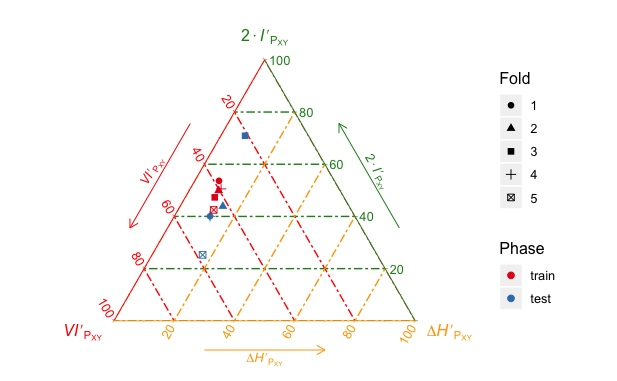
\includegraphics[width=1\linewidth]{Figuras_tfg/ET_knn_Ionosphere_auto}
	\caption{Entropy Triangle in Knn in Ionosphere using the Autoencoder}
	\label{fig:figure_Knn_Ionosphere_ET_Auto}
\end{figure}

\begin{figure}[H]
	\centering
	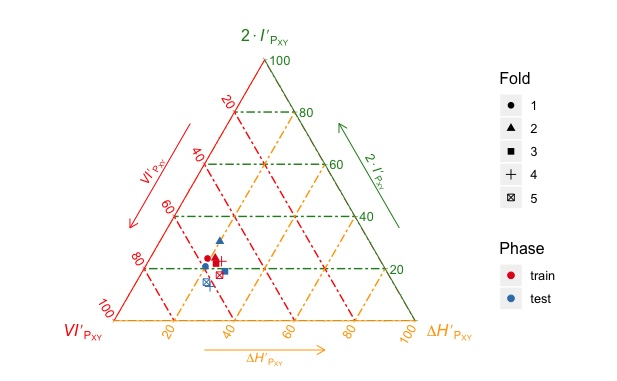
\includegraphics[width=1\linewidth]{Figuras_tfg/ET_knn_Ionosphere_pca}
	\caption{Entropy Triangle in Knn in Ionosphere using the PCA}
	\label{fig:figure_Knn_Ionosphere_ET_PCA}
\end{figure}

\begin{figure}[H]
	\centering
	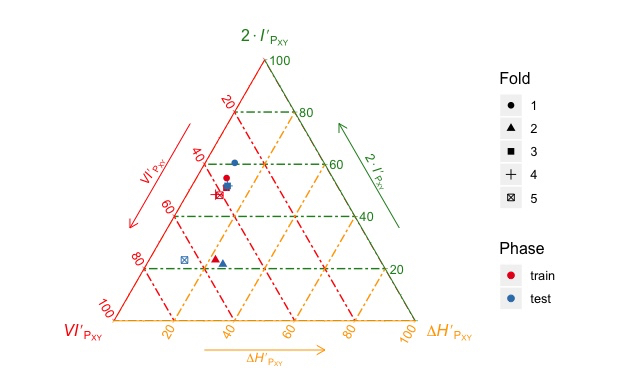
\includegraphics[width=1\linewidth]{Figuras_tfg/ET_mlp_Ionosphere_auto}
	\caption{Entropy Triangle in the MLP in Ionosphere using the Autoencoder}
	\label{fig:figure_MLP_Ionosphere_ET_Auto}
\end{figure}

\begin{figure}[H]
	\centering
	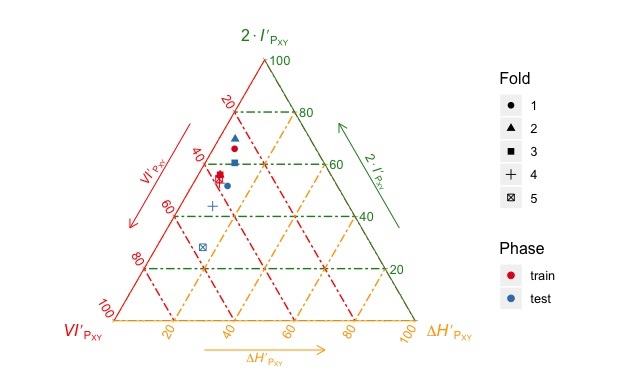
\includegraphics[width=1\linewidth]{Figuras_tfg/ET_mlp_Ionosphere_pca}
	\caption{Entropy Triangle in the MLP in Ionosphere using the PCA}
	\label{fig:figure_MLP_Ionosphere_ET_PCA}
\end{figure}

\begin{figure}[H]
	\centering
	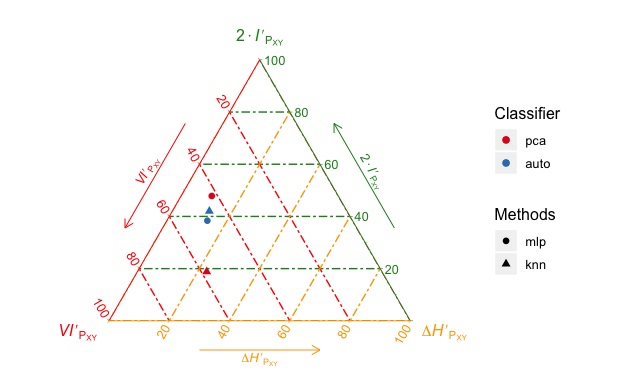
\includegraphics[width=1\linewidth]{Figuras_tfg/ET_Total_Ionosphere}
	\caption{Entropy Triangle in Ionosphere with the total test fold value}
	\label{fig:figure_Total_Ionosphere_ET}
\end{figure}



















	% COMENZAR A ESCRIBIR EL TRABAJO



%----------
%	BIBLIOGRAFÍA
%----------	

%\nocite{*} % Si quieres que aparezcan en la bibliografía todos los documentos que la componen (también los que no estén citados en el texto) descomenta está lína



\clearpage
\addcontentsline{toc}{chapter}{Bibliography}
%- Autoencoder bibliography (1980s) D.E. Rumelhart, G.E. Hinton, and R.J. Williams. Learning internal representations by error propagation. In Parallel Distributed Processing. Vol 1: Foundations. MIT Press, Cambridge, MA, 1986.

\printbibliography



%----------
%	ANEXOS
%----------	

% Si tu trabajo incluye anexos, puedes descomentar las siguientes líneas
%\chapter* {Appendix x}
%\pagenumbering{gobble} % Las páginas de los anexos no se numeran



\end{document}